\documentclass[10pt]{article}
\usepackage[spanish]{babel}
\usepackage[utf8]{inputenc}
\usepackage{graphicx}
\usepackage{hyperref}
\usepackage[lmargin=2cm, rmargin=2cm, top=2cm, bottom=2 cm]{geometry}
\usepackage{fancyhdr}
\pagestyle{fancy}

\usepackage[table,xcdraw]{xcolor}
\fancyhead{}
\fancyhead[R]{Facultad de Ingeniería UNAM\\ van der Werff Pieter}
\fancyhead[L]{
\includegraphics[height=0.75cm]{img/escudofi_negro.jpg}}
\usepackage{animate}
\usepackage{enumerate}
\usepackage{float}
\usepackage{url}
\usepackage{karnaugh-map}
\usepackage{float}
\usepackage{subcaption}

\fancyfoot{}
\fancyfoot[R]{Página \thepage \hspace{0.02 cm}}
\renewcommand{\headrulewidth}{0.9pt}
\renewcommand{\footrulewidth}{0.5pt}

\usepackage{listings}
\usepackage{xcolor}

\usepackage{verbatim}
\usepackage{minted}

%New colors defined below
\definecolor{codegreen}{rgb}{0,0.6,0}
\definecolor{codegray}{rgb}{0.5,0.5,0.5}
\definecolor{codepurple}{rgb}{0.58,0,0.82}
\definecolor{backcolour}{rgb}{0.95,0.95,0.92}

\definecolor{dkgreen}{rgb}{0,0.6,0}
\definecolor{gray}{rgb}{0.5,0.5,0.5}
\definecolor{mauve}{rgb}{0.58,0,0.82}

%Code listing style named "mystyle"
\lstdefinestyle{mystyle}{
  backgroundcolor=\color{backcolour},   commentstyle=\color{codegreen},
  keywordstyle=\color{magenta},
  numberstyle=\tiny\color{codegray},
  stringstyle=\color{codepurple},
  basicstyle=\ttfamily\footnotesize,
  breakatwhitespace=false,         
  breaklines=true,                 
  captionpos=b,                    
  keepspaces=true,                 
  numbers=left,                    
  numbersep=5pt,                  
  showspaces=false,                
  showstringspaces=false,
  showtabs=false,                  
  tabsize=2
}

\lstset{style=mystyle}

\begin{document}
\date{}  
\begin{titlepage}
\begin{center}
    \vspace*{\baselineskip}
    
    {
    \bf\fontsize{19}{0}{\selectfont{UNIVERSIDAD NACIONAL AUTONOMA DE MÉXICO}}\\[0.5cm]
    \fontsize{11}{0}{FACULTAD DE INGENIERÍA}
    }
    
    %\vspace*{0.5\baselineskip}
    %{
    %\bf\fontsize{11}{0}{\selectfont{ESCUELA DE INFORMÁTICA Y TELECOMUNICACIONES}}\\[0.35cm]
    %}
    
    \vspace*{\baselineskip}
    
\includegraphics[scale=0.50]{img/escudofi_negro.jpg}
    \vspace*{3\baselineskip}
     \hrule height 0.5pt
    \vspace{1mm}
    \hrule height 1.5pt
    \vspace*{1\baselineskip}
   
    {
    \bf\fontsize{15}{0}{\selectfont{Inteligencia Artificial \\[0.3cm] Proyecto Final}}
    }
    \vspace*{1\baselineskip}
    \hrule height 0.5pt
    \vspace{1mm}
    \hrule height 1.5pt
    
    
    \vspace*{4.5\baselineskip}
    
    {
     \bf\fontsize{14}{0}{\selectfont{Profesor:\\[0.3cm]
}}

\bf\fontsize{14}{0}{\selectfont{Dr. Guillermo Molero Castillo\\[0.5cm]
}}


   

   \bf\fontsize{14}{0}{\selectfont{Estudiante:\\[0.3cm]}}
   \bf\fontsize{14}{0}{\selectfont{Pieter Alexander van der Werff Vargas}
   }
    
    \vfill
    Grupo 3  \hfill Semestre 2022-1
    
\end{center}
\end{titlepage}
\vspace*{\baselineskip}
\tableofcontents 
\setcounter{page}{0}
\thispagestyle{empty}
\newpage


\section{Introducción}

\begin{abstract}
    Este trabajo es una compilación de distintos algoritmos de inteligencia artificial, mediante el cual se da a la tarea de exponer la utilidad y el funcionamiento de cada uno de los mismos. Estos fueron desarrollados haciendo uso de la herramienta Streamlit, la cual se hablará más a fondo a continuación.
\end{abstract}

Es interesante estudiar de forma teórica el funcionamiento de distintos algoritmos de inteligencia artificial, sean de tipo supervisado, de regresión o clasificación; como es el caso de Regresión Logística y árboles de regresión y decisión; o no supervisados: como lo son el algoritmo apriori y los distintos algoritmos de clustering. Sin embargo, es importante tener en cuenta un contexto más real de la utilidad que se tiene para cada algoritmo, ya sea para ayudar en compras en línea o selección de un catálogo de películas utilizando apriori; hasta aplicaciones más importantes como son en la medicina el diagnóstico de un tumor de mama, para saber si es benigno o maligno, utilizando algoritmos de clasificación. Para esto se realizará una interfaz gráfica, mediante una página web, en la cual se visualizará un ejemplo de cada implementación que tenga uno de los algoritmos estudiados; o bien se podrá acceder a un \textit{Modo Avanzado}, mediante el cual se podrán observar las métricas del algoritmo o realizar ajuste de parámetros para su funcionamiento.

\subsection{Tecnología Usada - e instalación}
    Para el desarrollo de este proyecto, se recurrió a la plataforma \href{https://streamlit.io/}{Streamlit}, debido a su versatilidad y facilidad para incorporar código de lenguaje Python para el backend del sistema; así como herramientas visuales como tablas y gráficas, las cuales se generan en una página web para su visualización sencilla.
    
    \begin{figure}[ht!]
    \centering
    
\includegraphics[height= 1.5cm]{img/streamlit.png}
    %\caption{Ejemplo de proyecto Sreamlit}
    \label{fig:StreamlitLogo}
    \end{figure}
    
    Para realizar su instalación, se requiere primeramente tener alguna versión de Python reciente instalada en el sistema e instalar \textit{PIP}. En este caso se trabajó en un sistema operativo Ubuntu Linux, por lo cual se realiza utilizando la terminal.
    
    \begin{verbatim}
        sudo apt-get install python3-pip
    \end{verbatim}
    
    Una vez realizado esto, se instala un entorno para pip.
    
    \begin{verbatim}
        pip3 install pipenv
    \end{verbatim}
    
    Ahora se accede a la ubicación para nuestro proyecto, entramos a un ambiente de pip y una vez ahí instalamos la libreria \textit{streamlit}
    
    \begin{verbatim}
        cd ProyectoFinal
        pipenv shell
        pip install streamlit
    \end{verbatim}
    
    Una vez instalado streamlit, podemos acceder a nuestro proyecto utilizando el comando \textit{streamlit}, dentro de un ambiente de pip, utilizando como parámetros el nombre del archivo con el cual trabajamos}
    
    \begin{verbatim}
        streamlit run ProyectoFinal.py
    \end{verbatim}
    
    El archivo de python con el que trabajemos requiere importar la biblioteca \textit{streamlit} para su funcionamiento, la cual además nos proporciona diversas funciones, las cuales son útiles para visualizar el contenido en la página web que genera al iniciar la instancia del proyecto
    
    \begin{minted}[mathescape, linenos]{python}
    import pandas as pd
    import numpy as np
    import matplotlib.pyplot as plt
    import streamlit as st
    
    # Ejemplo de mostrar texto en Streamlit
    st.write('Hola Mundo')
    
    # Ejemplo mostrar matriz de datos
    lista = [['Dato 1', 'Dato A'], ['Dato 2', 'Dato B']]
    datos = pd.DataFrame(lista)
    st.dataframe(datos)
    
    # Ejemplo mostrar gráfica
    fig, ax = plt.subplots()
    ax.plot(range(0,10))
    st.pyplot(fig)
    \end{minted}
    
    Se observa en la figura \ref{fig:ejStreamlit} que se tiene una gran facilidad en cuanto a la impresión de los distintos elementos visuales para realizar la interfaz gráfica para nuestros algoritmos y no es necesario hacer uso de código en HTML; aunque sí es posible modificar código de HTML si se requiere modificar o personalizar de mayor manera nuestra página web.
    
    \begin{figure}[ht!]
    \centering
    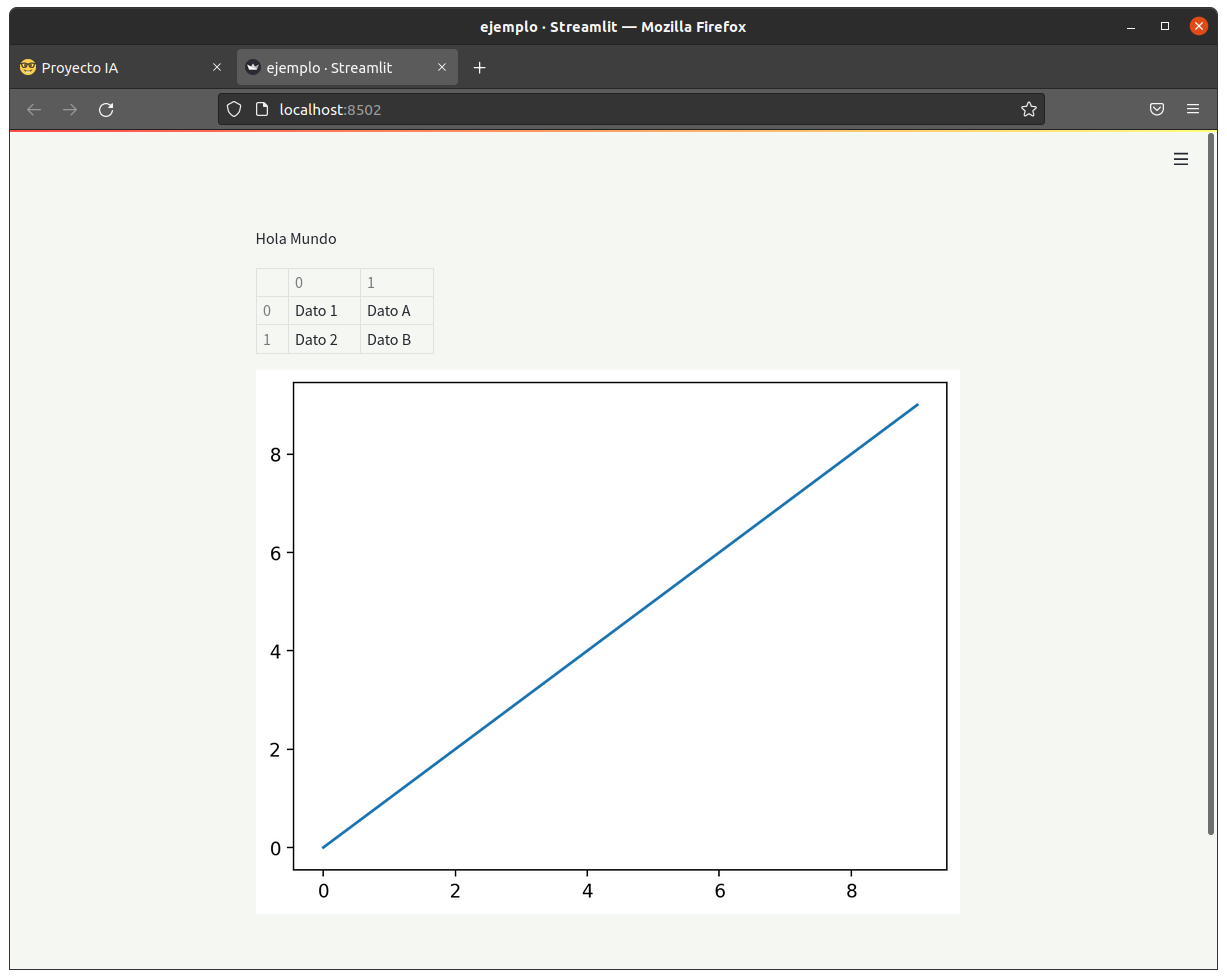
\includegraphics[width=10cm]{img/ejStreamlit.png}
    \caption{Ejemplo de proyecto Sreamlit}
    \label{fig:ejStreamlit}
    \end{figure}
    
\newpage
    
\subsection{Diseño General}

    \begin{figure}[ht!]
        \centering
        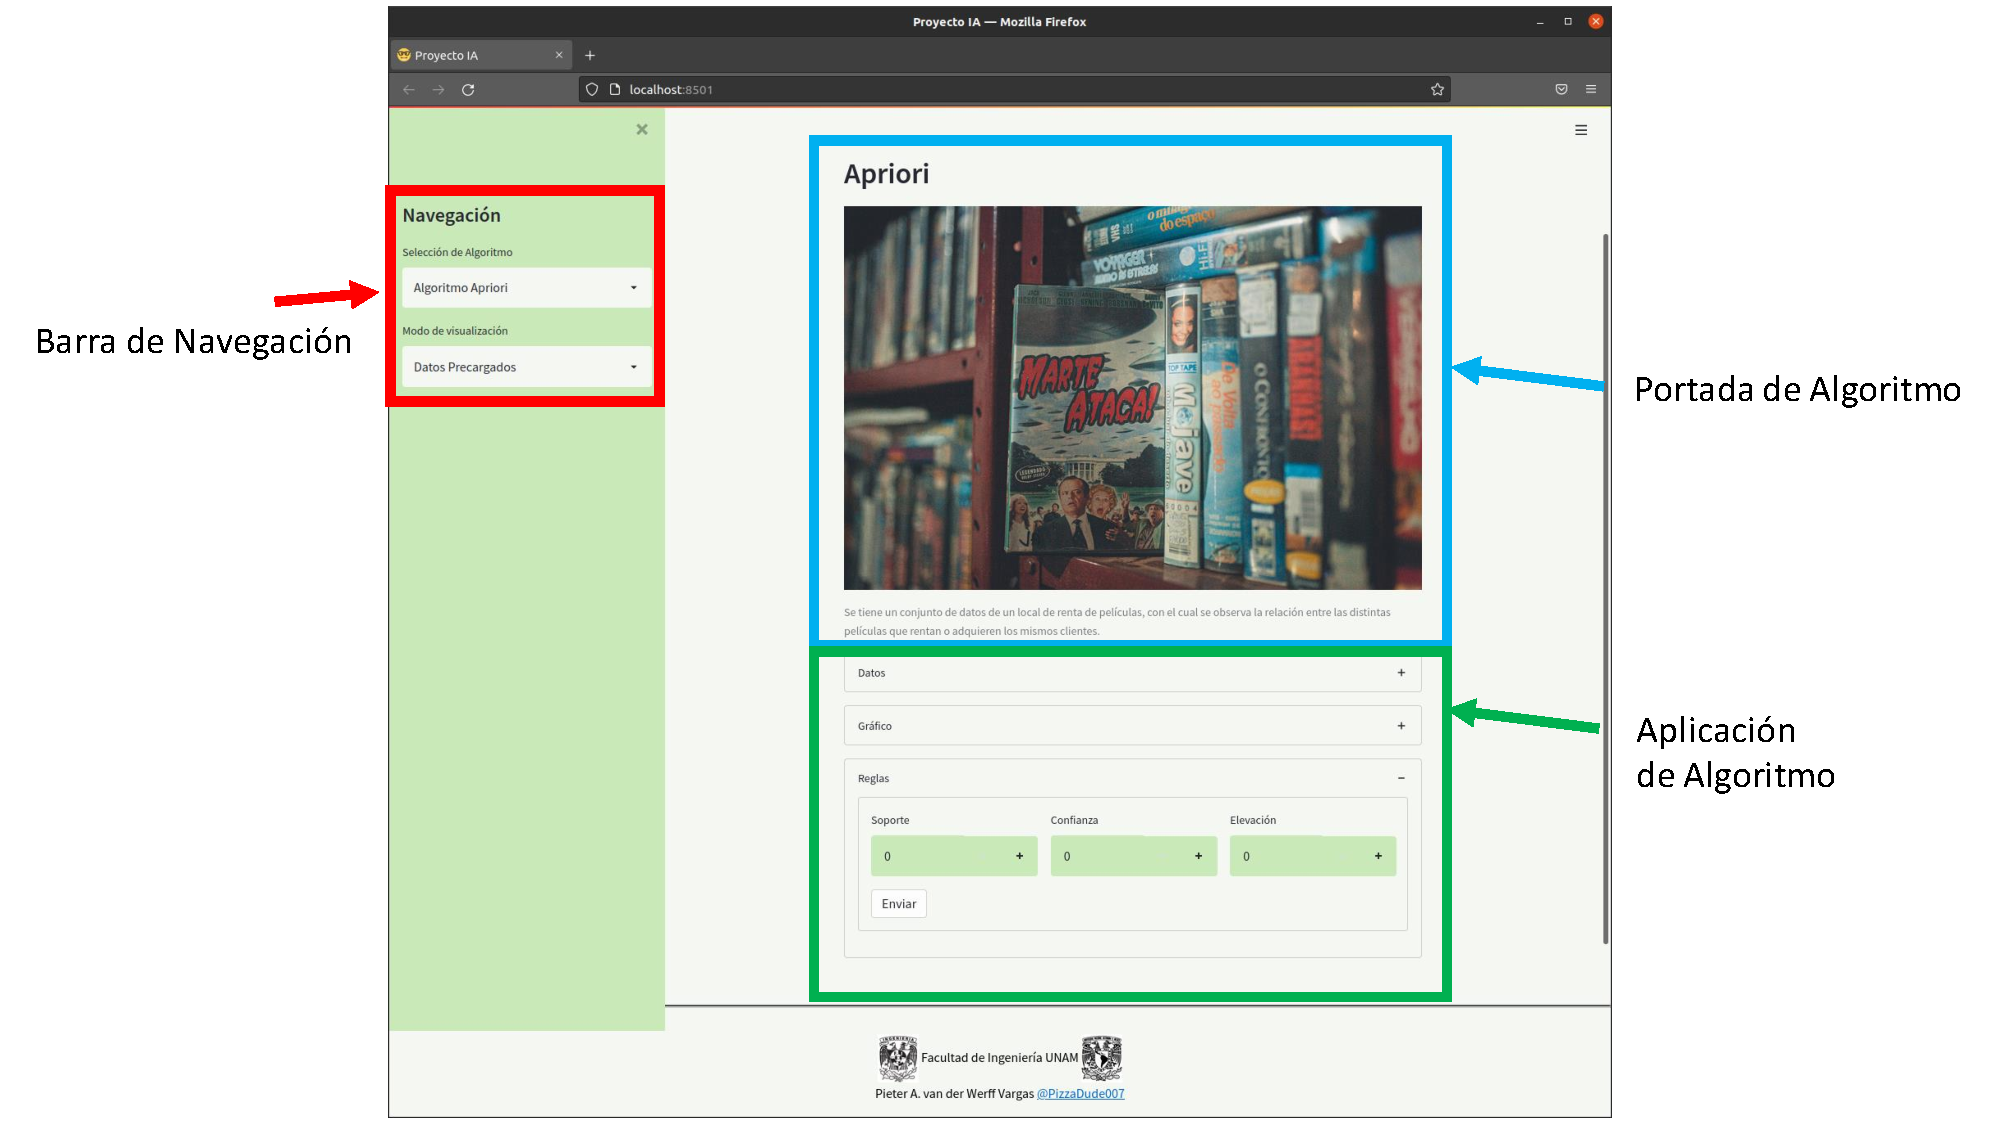
\includegraphics[height=7cm]{img/Ejemplo.pdf}
        \caption{Algoritmo Apriori}
        \label{fig:Ejemplo}
    \end{figure}
    
    Streamlit hace uso de una pestaña izquierda, la cual se le llama \textit{sidebar}, esta barra puede ser de utilidad como menú, ya que se puede esconder o expander dependiendo de si se requiera o no. Por esta razón se utlizó como barra de navegación, como se muestra en la figura \ref{Ejemplo}. Aquí se seleccionará el algoritmo o módulo el cual se quiera revisar, además de la selección de \textit{Modo de visualización}; siendo este por defecto \textit{Datos Precargados} el cual nos mostrará una breve introducción del módulo que se está utilizando además de una manera rápida de utilizar la implementación de ese modelo. En cambio, si se selecciona la opción \textit{Modo Avanzado}, se tendrá acceso a una mayor cantidad de parámetros para configurar el funcionamiento de cada algoritmo, además de que se mostrará el porcentaje de exactitud y otras métricas acorde al modelo que se revise. Por otra parte, si se utiliza el \textit{Modo Avanzado}, se tendrá que cargar el archivo a leer manualmente.\newline
    
    Independientemente del modo de visualización que se esté utilizando cada implementación tiene una serie de contenedores que se pueden colapsar o desplegar si se quiere ver más información de dicho modelo o del conjunto de datos que se haya cargado, ya sea desde un archivo o se tenga precargado. El primero de estos siempre será la matriz que contiene el conjunto de datos del archivo que se haya cargado, ya sea internamente o por el usuario.\newline 
    
    Por último se tiene un pie de página, el cual se mantiene persistente independientemente del algoritmo o tipo de visualización que se esté utilizando. Este pie de página requirió de una modificación a la parte de HTML del proyecto, debido a que la herramienta Streamlit no soporta realizar algo así de manera nativa.

\newpage
\section{Desarrollo}

\subsection{Algoritmo Apriori}

    \begin{figure}[H]
    
    \begin{subfigure}{0.5\textwidth}
    \centering
    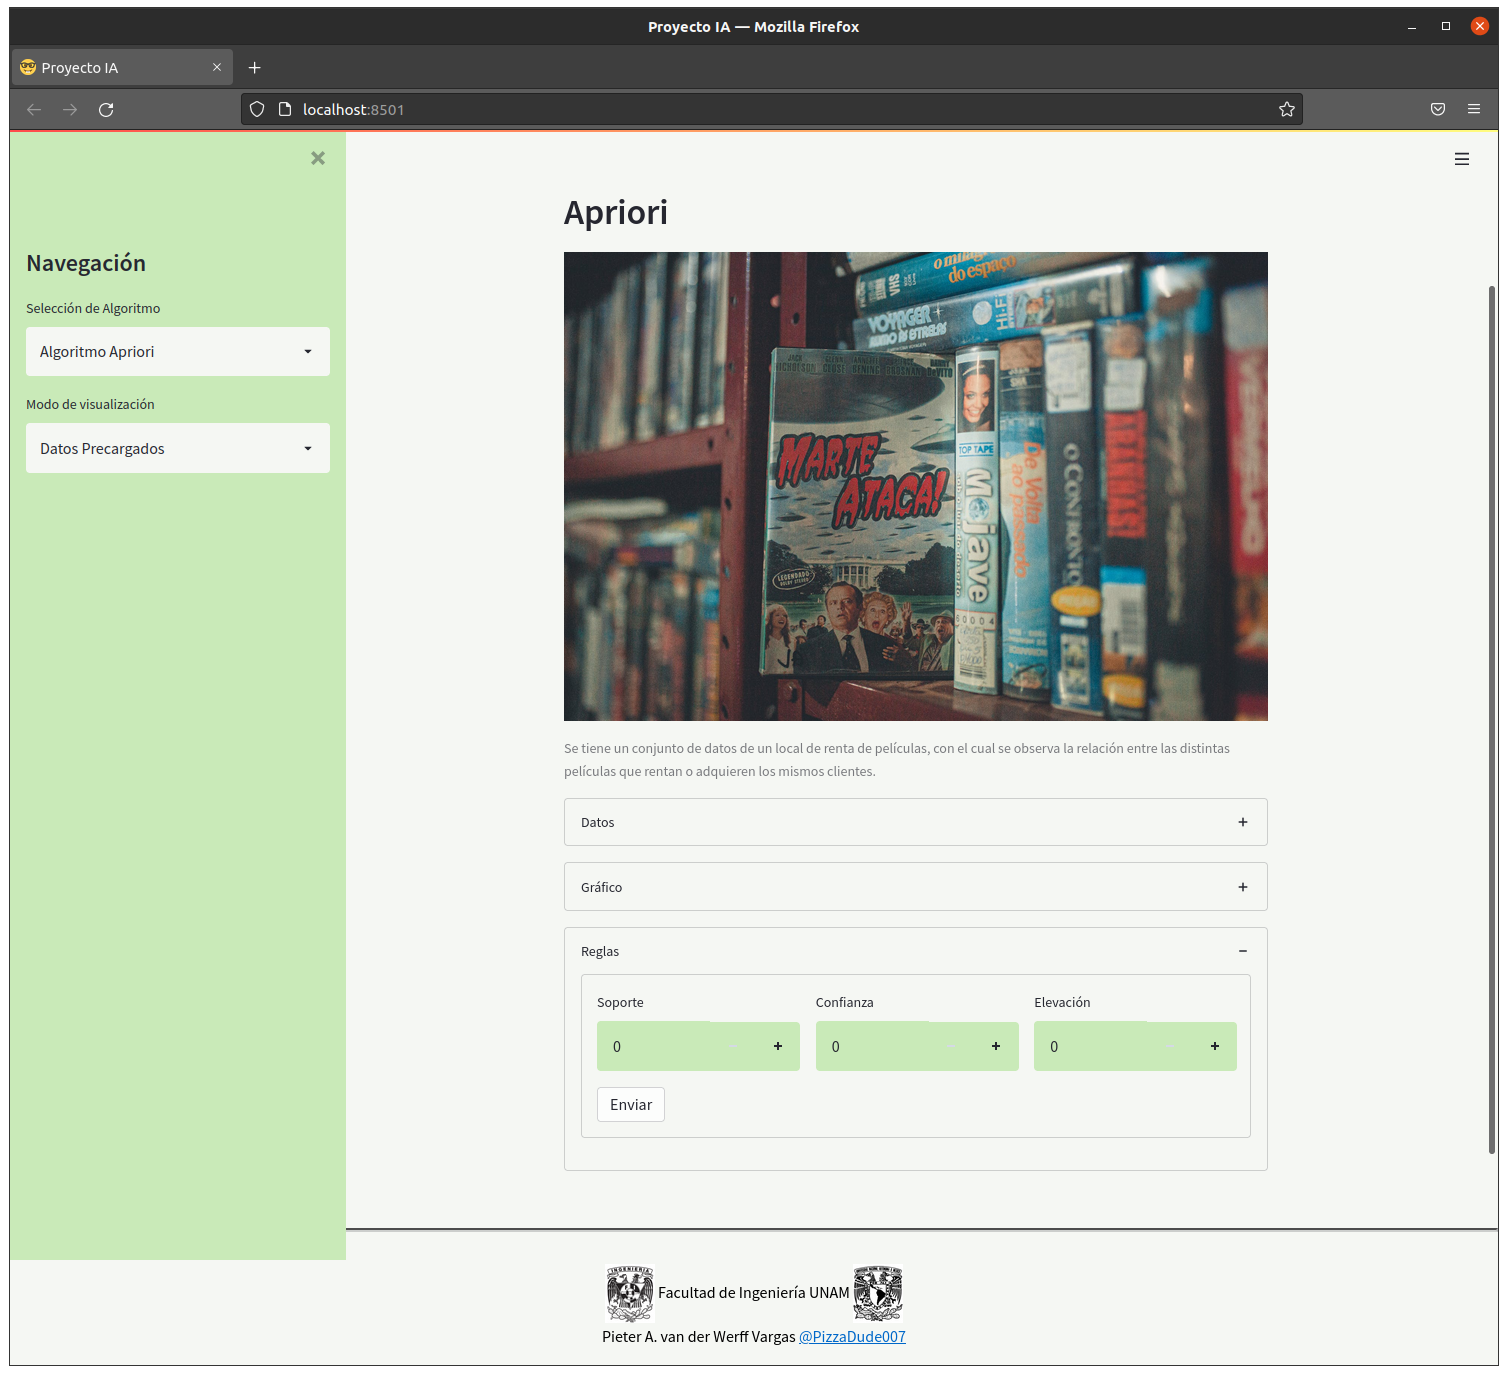
\includegraphics[height=6cm]{img/Apriori_DP.png} 
    \caption{Datos Precargados}
    \label{fig:AprioriDP}
    \end{subfigure}
    \begin{subfigure}{0.5\textwidth}
    \centering
    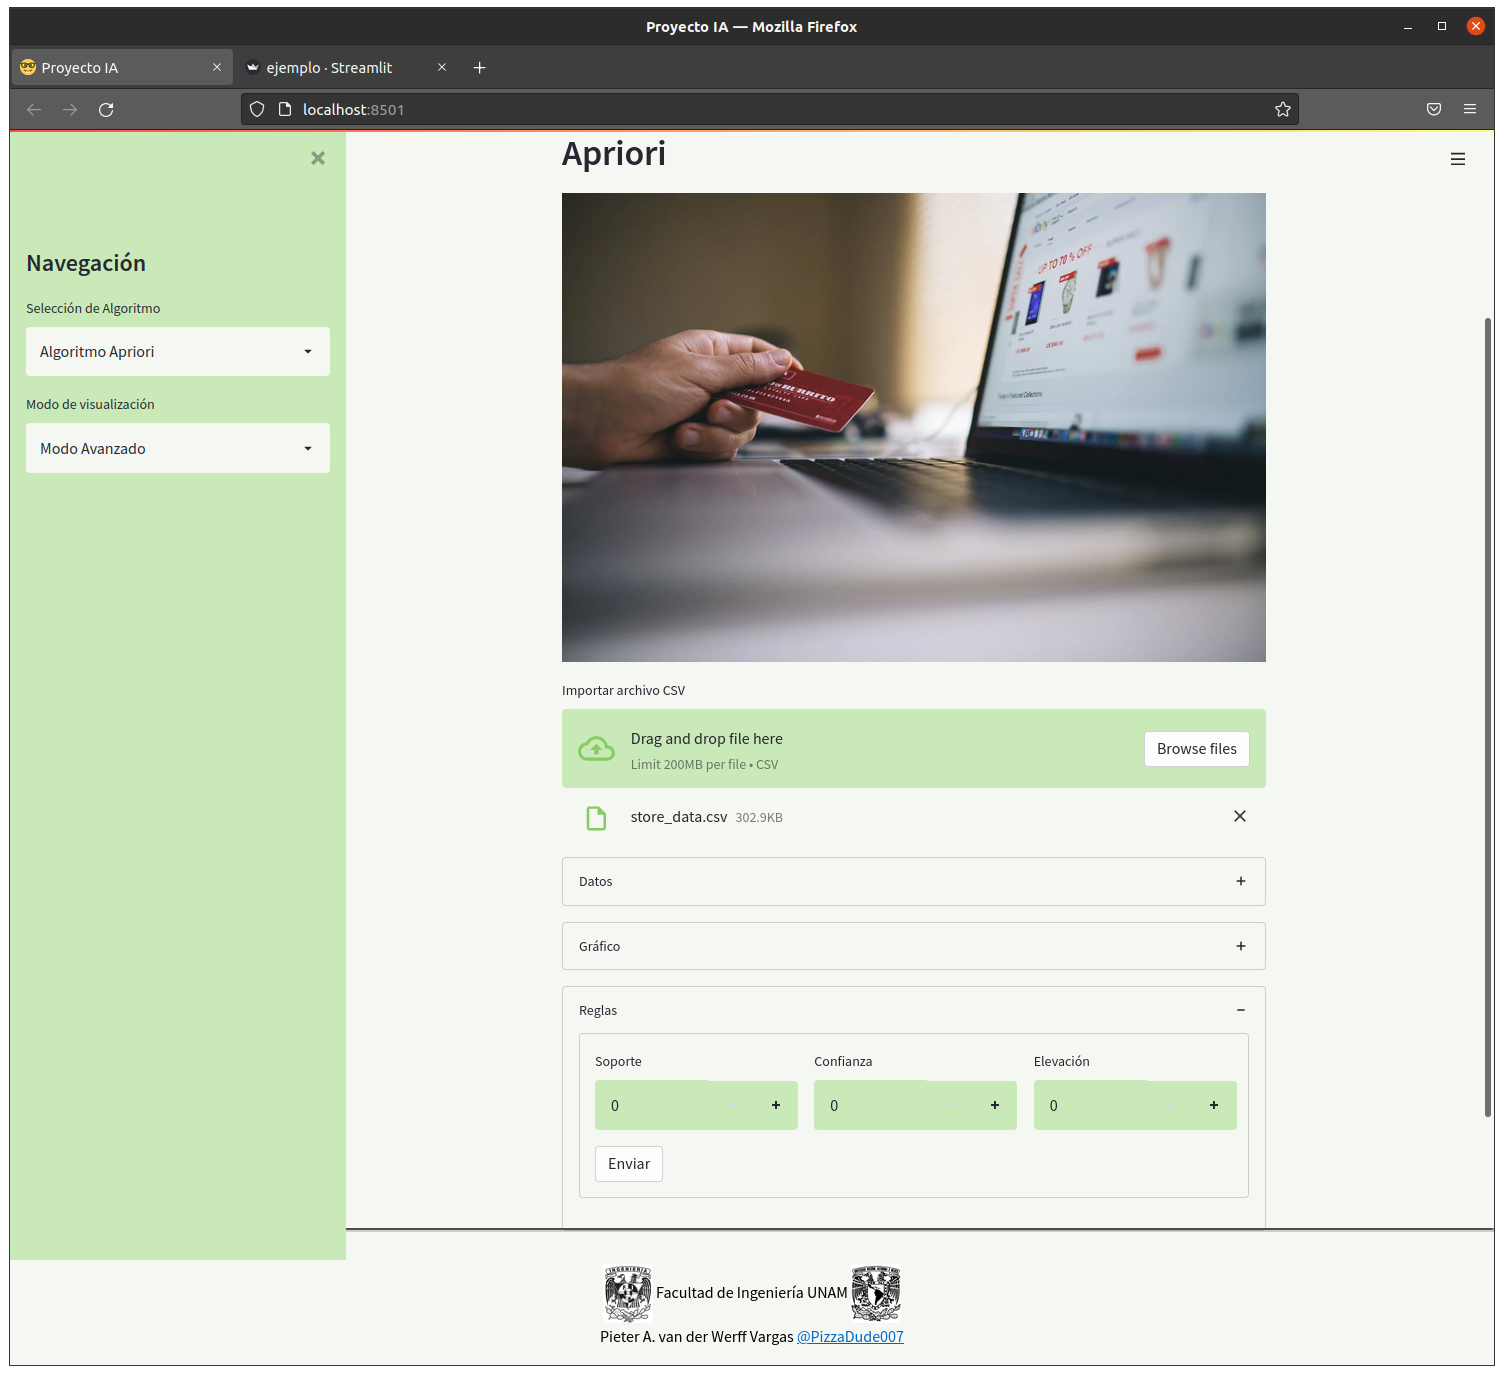
\includegraphics[height=6cm]{img/AprioriMA.png}
    \caption{Modo Avanzado}
    \label{fig:AprioriMC}
    \end{subfigure}
    
    \caption{Algoritmo Apriori}
    \label{fig:Apriori}
    \end{figure}
    
    Si se utiliza el modo de visualización de \textit{Datos Precargados}, se utilizará una fuente de datos de un local de renta de películas, de forma que se pueda establecer directamente los parámetros de soporte, confianza y elevación par visualizar una tabla en donde cada fila representará una regla distinta que se haya generado con este modelo. Además, en cualquiera de las formas de visualización se puede observar una gráfica con las transacciones de la fuente de datos que se haya proporcionado.
    
    \begin{figure}[H]
    \centering
    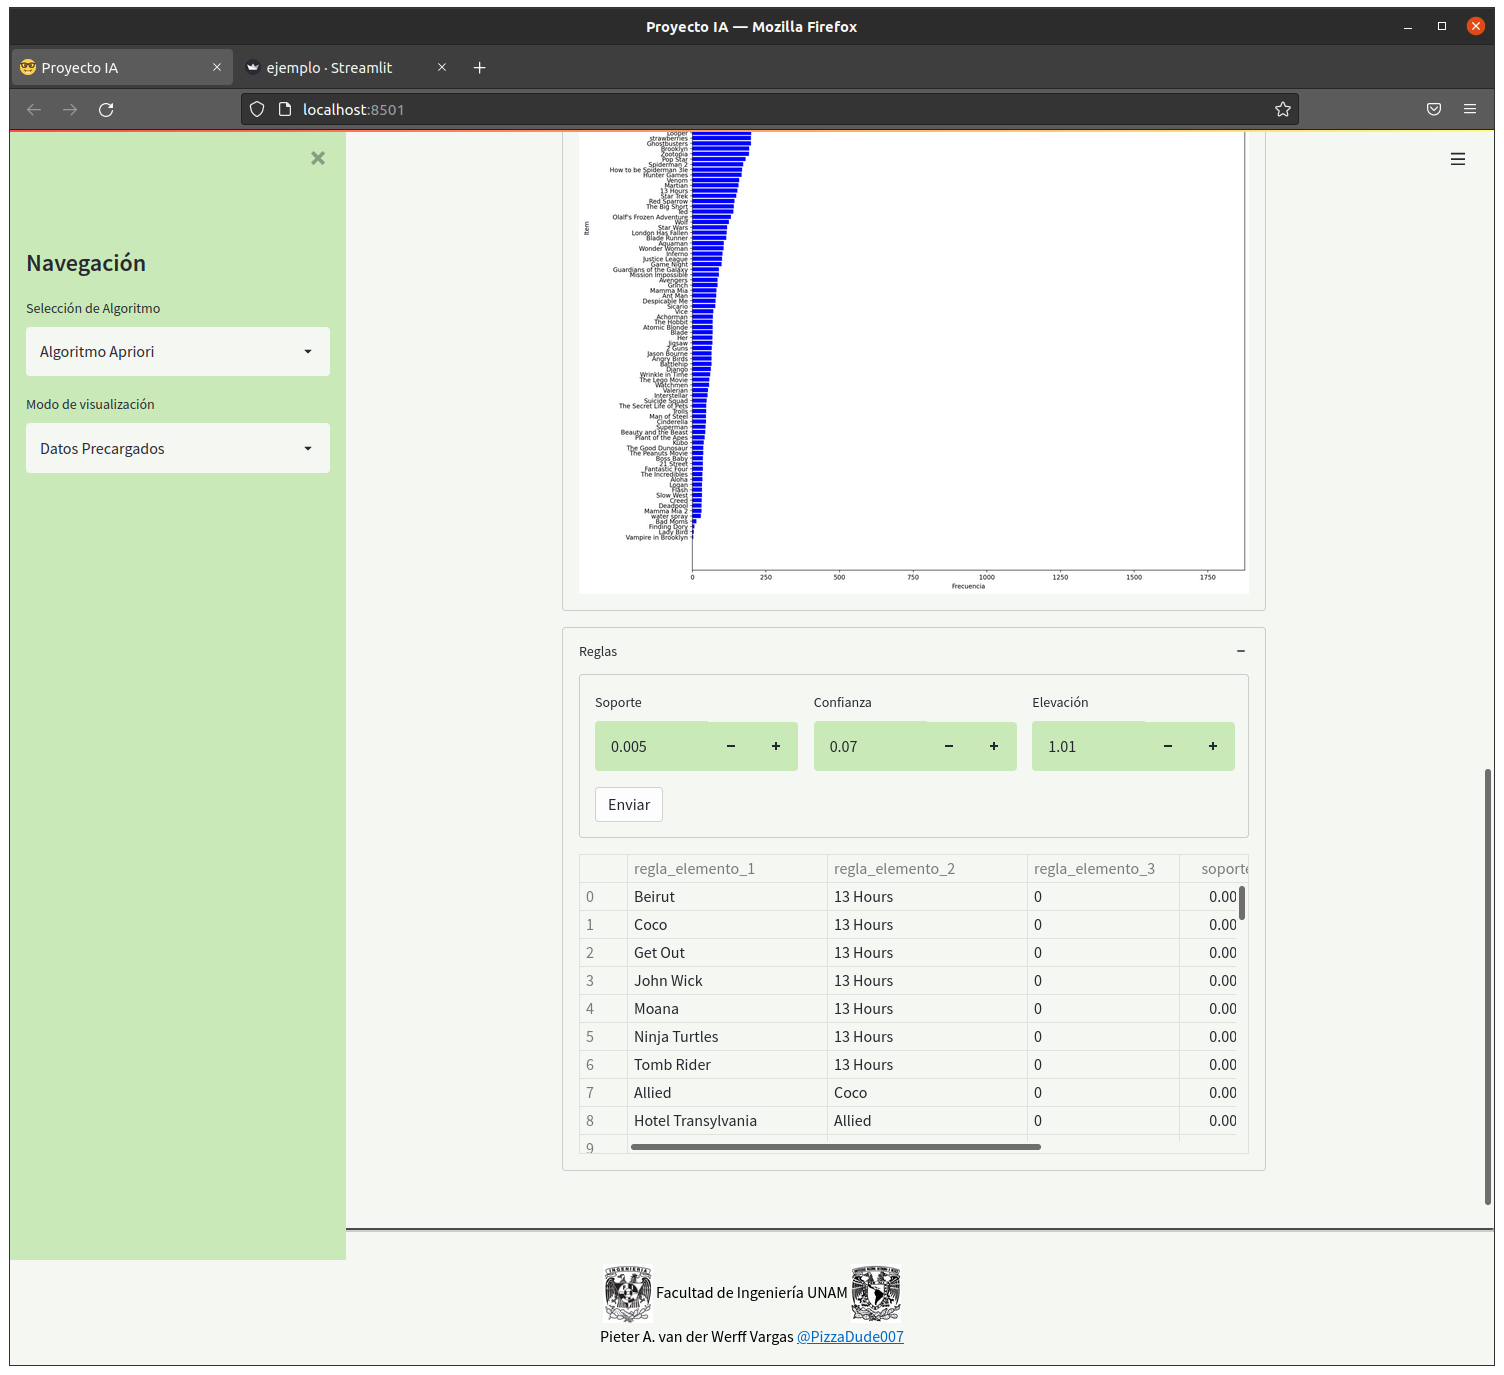
\includegraphics[height=6cm]{img/AprioriSal.png}
    \caption{Salida Apriori}
    \label{fig:AprioriSalida}
    \end{figure}

\subsection{Métricas de Distancia}

    \begin{figure}[H]
    
    \begin{subfigure}{0.5\textwidth}
    \centering
    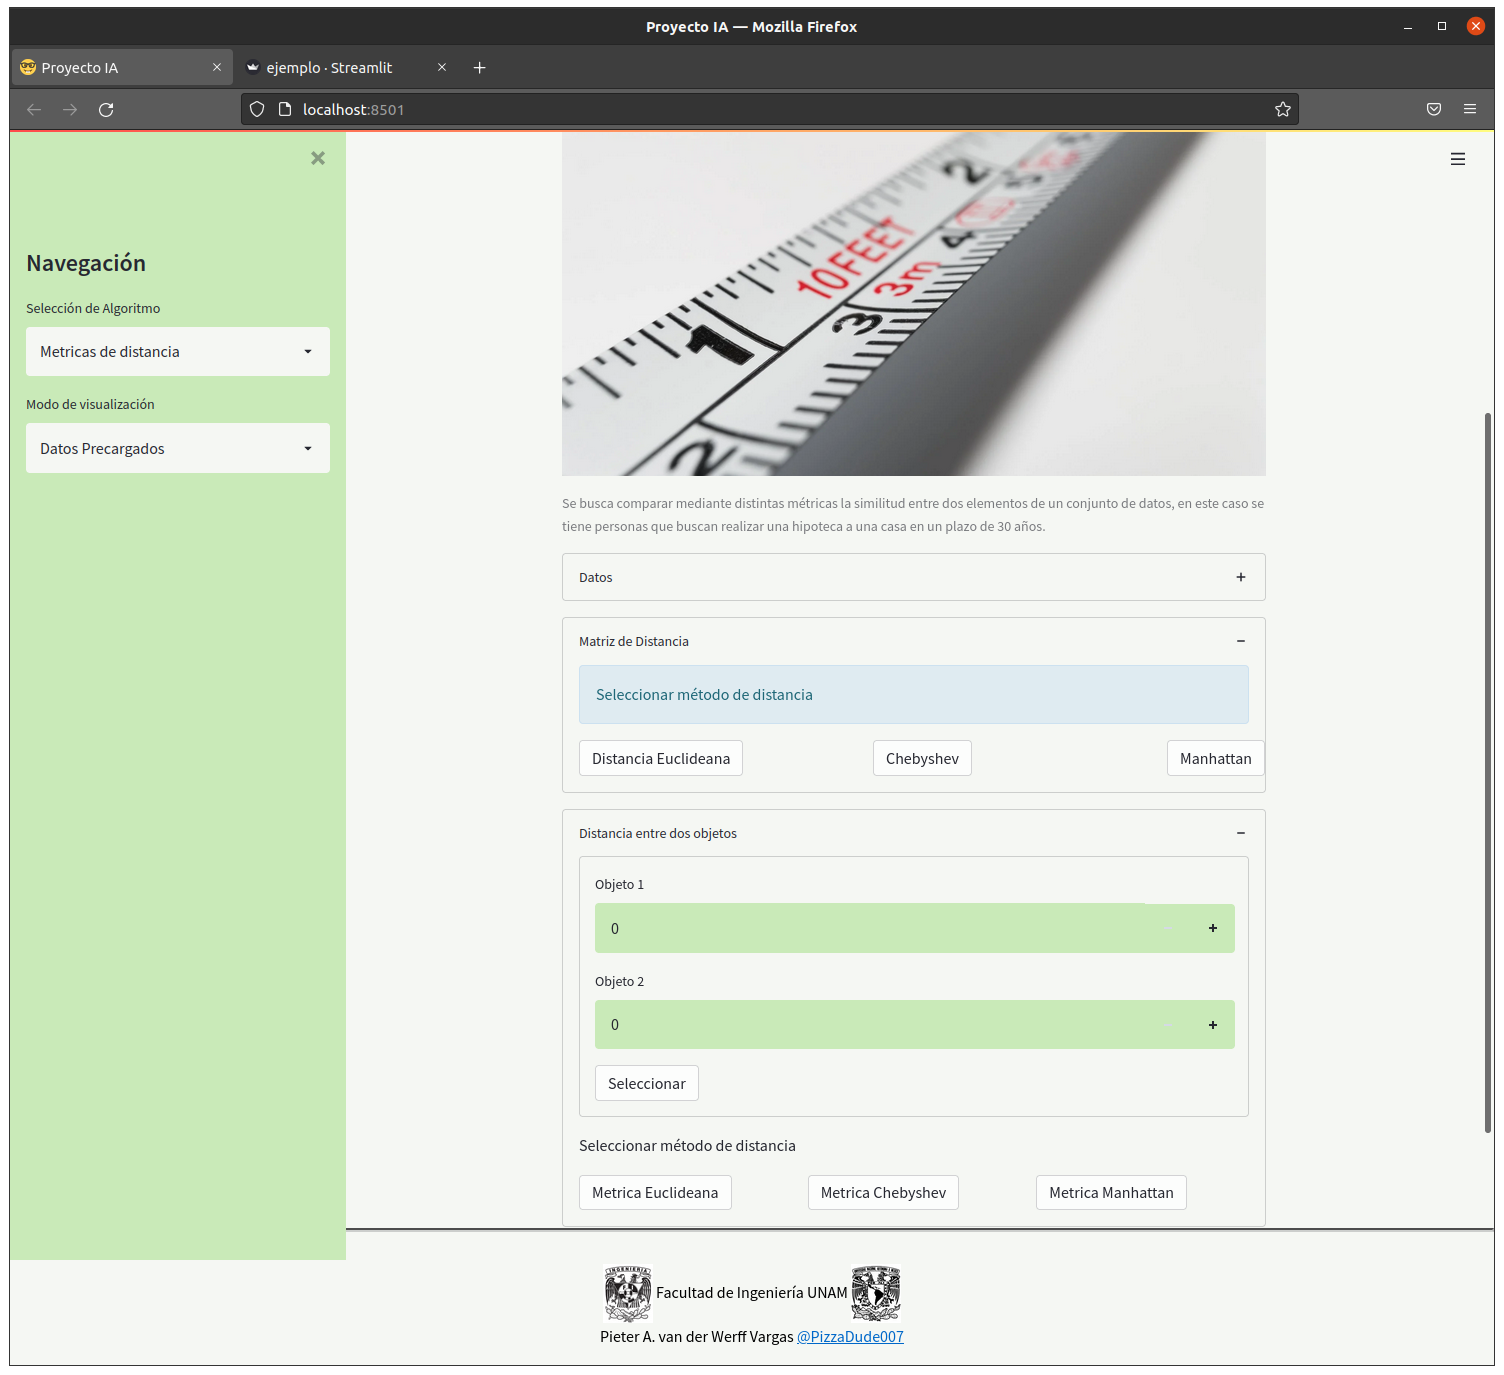
\includegraphics[height=6cm]{img/MetricasDP.png} 
    \caption{Datos Precargados}
    \label{fig:MetricasDP}
    \end{subfigure}
    \begin{subfigure}{0.5\textwidth}
    \centering
    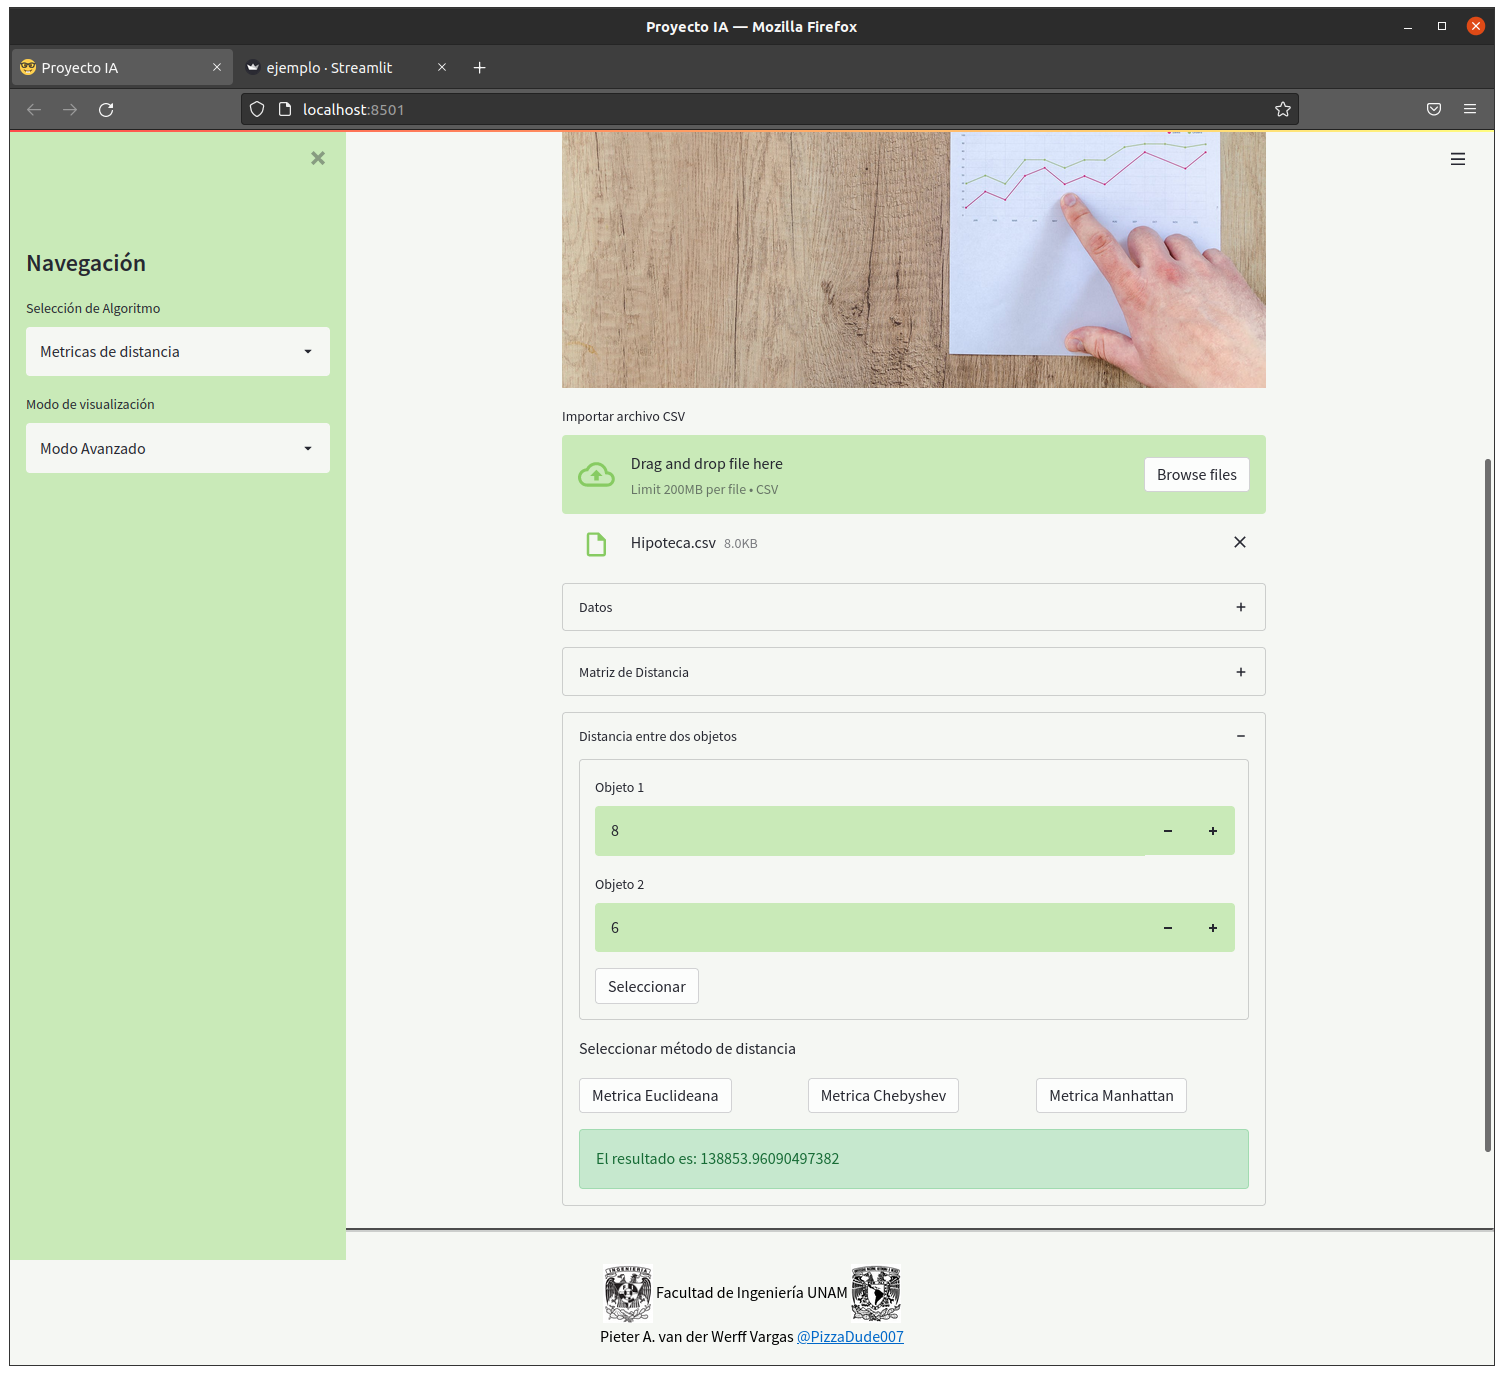
\includegraphics[height=6cm]{img/MetricasMA.png}
    \caption{Modo Avanzado}
    \label{fig:MetricasMC}
    \end{subfigure}
    
    \caption{Métricas de Distancia}
    \label{fig:MetricasDistancia}
    \end{figure}
    
    El módulo para Métricas de Distancia, es otro módulo sencillo, en el cual se tiene únicamente dos contenedores adicionales al de la matriz del conjunto de datos. En el primer bloque se puede seleccionar alguna de las métricas de distancia por mostrar una matriz, siendo esta matriz de tipo simétrica, en la cual se hayan ordenado los elementos de acuerdo con el conjunto de datos que se haya ingresado.\newline
    
    \begin{figure}[H]
    \centering
    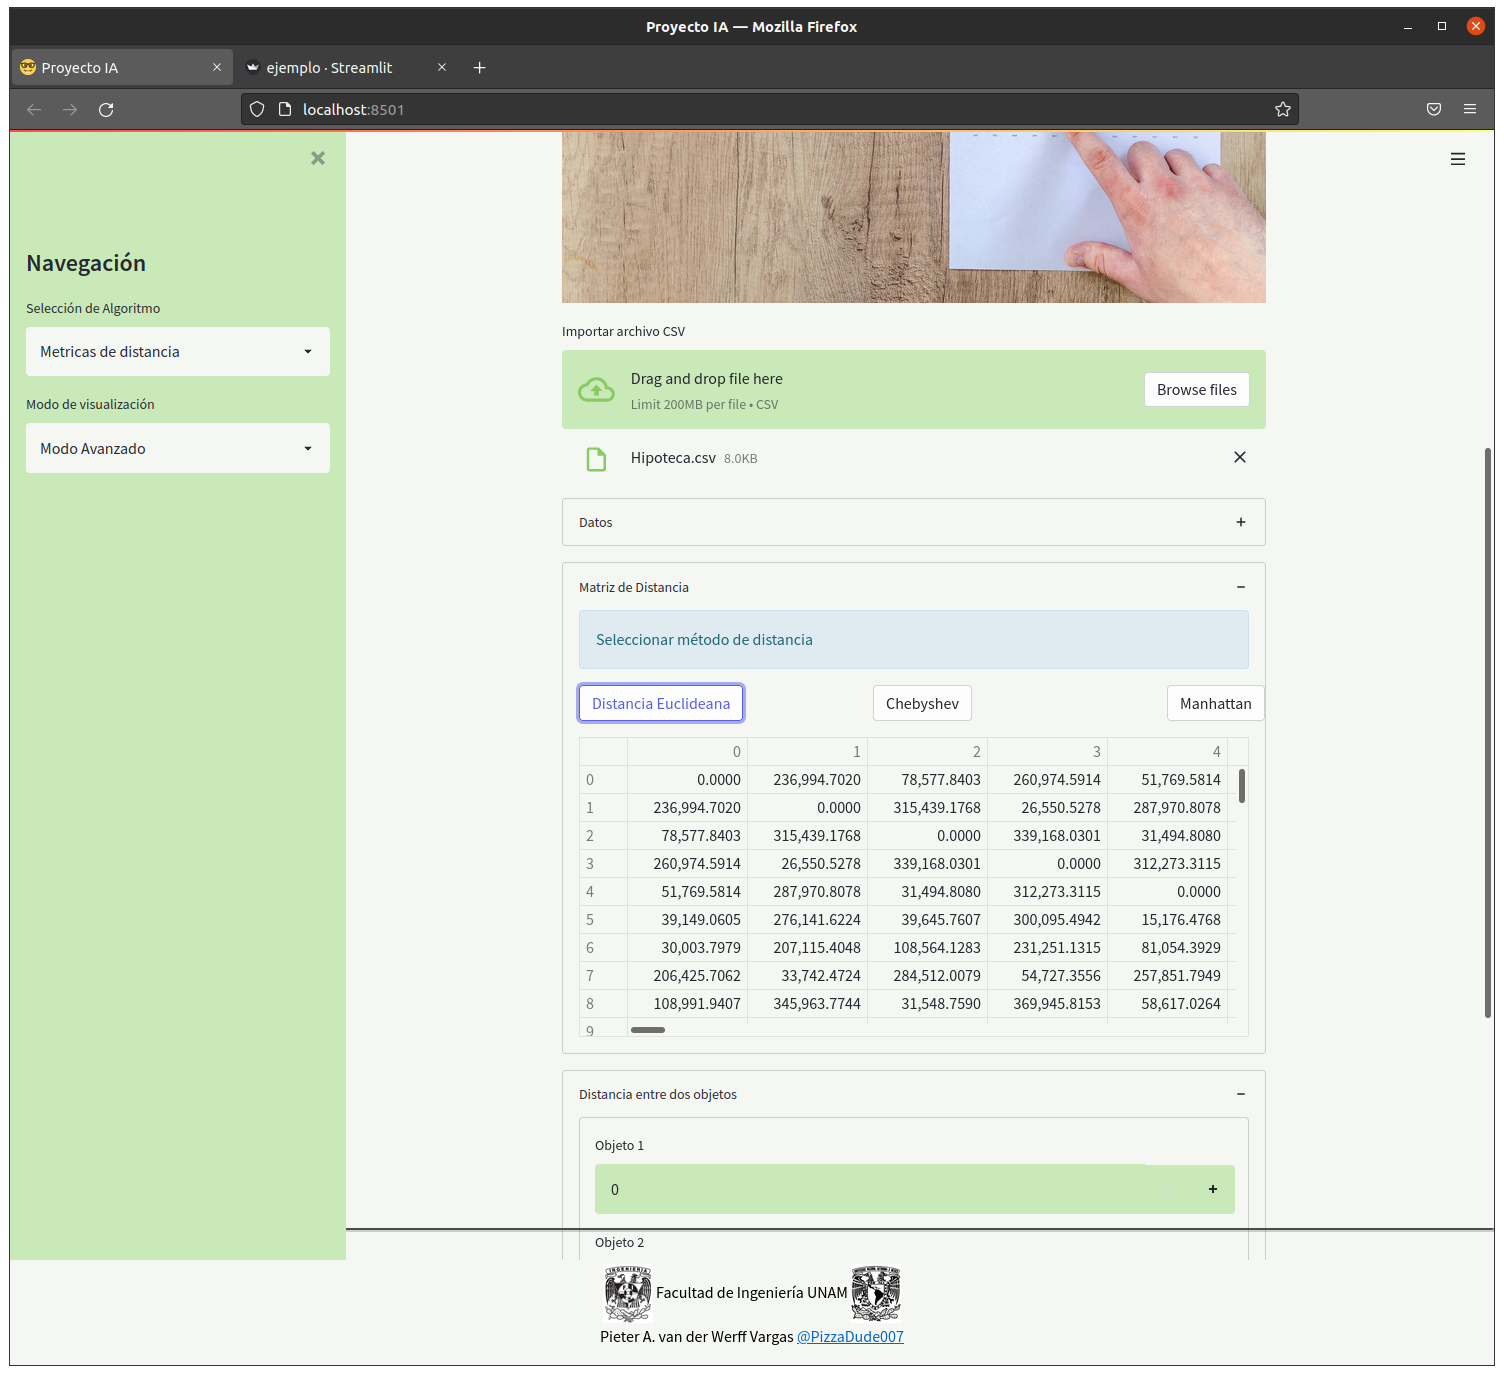
\includegraphics[height=6cm]{img/Metrica_salida.png}
    \caption{Matriz de Distancia}
    \label{fig:MetSalida}
    \end{figure}
    
    Por otro lado, en el segundo bloque se tiene un formulario por el cual se elige a dos objetos del conjunto de datos, para poder obtener su distancia; ya sea por medio de la métrica euclideana, Chebyshev o Manhattan. Aquí se deberá de elegir y cargar dos vectores antes de poder seleccionar algún método de distancia.\newline

\subsection{Módulo Clustering}

    \begin{figure}[H]
    \begin{subfigure}{0.5\textwidth}
    \centering
    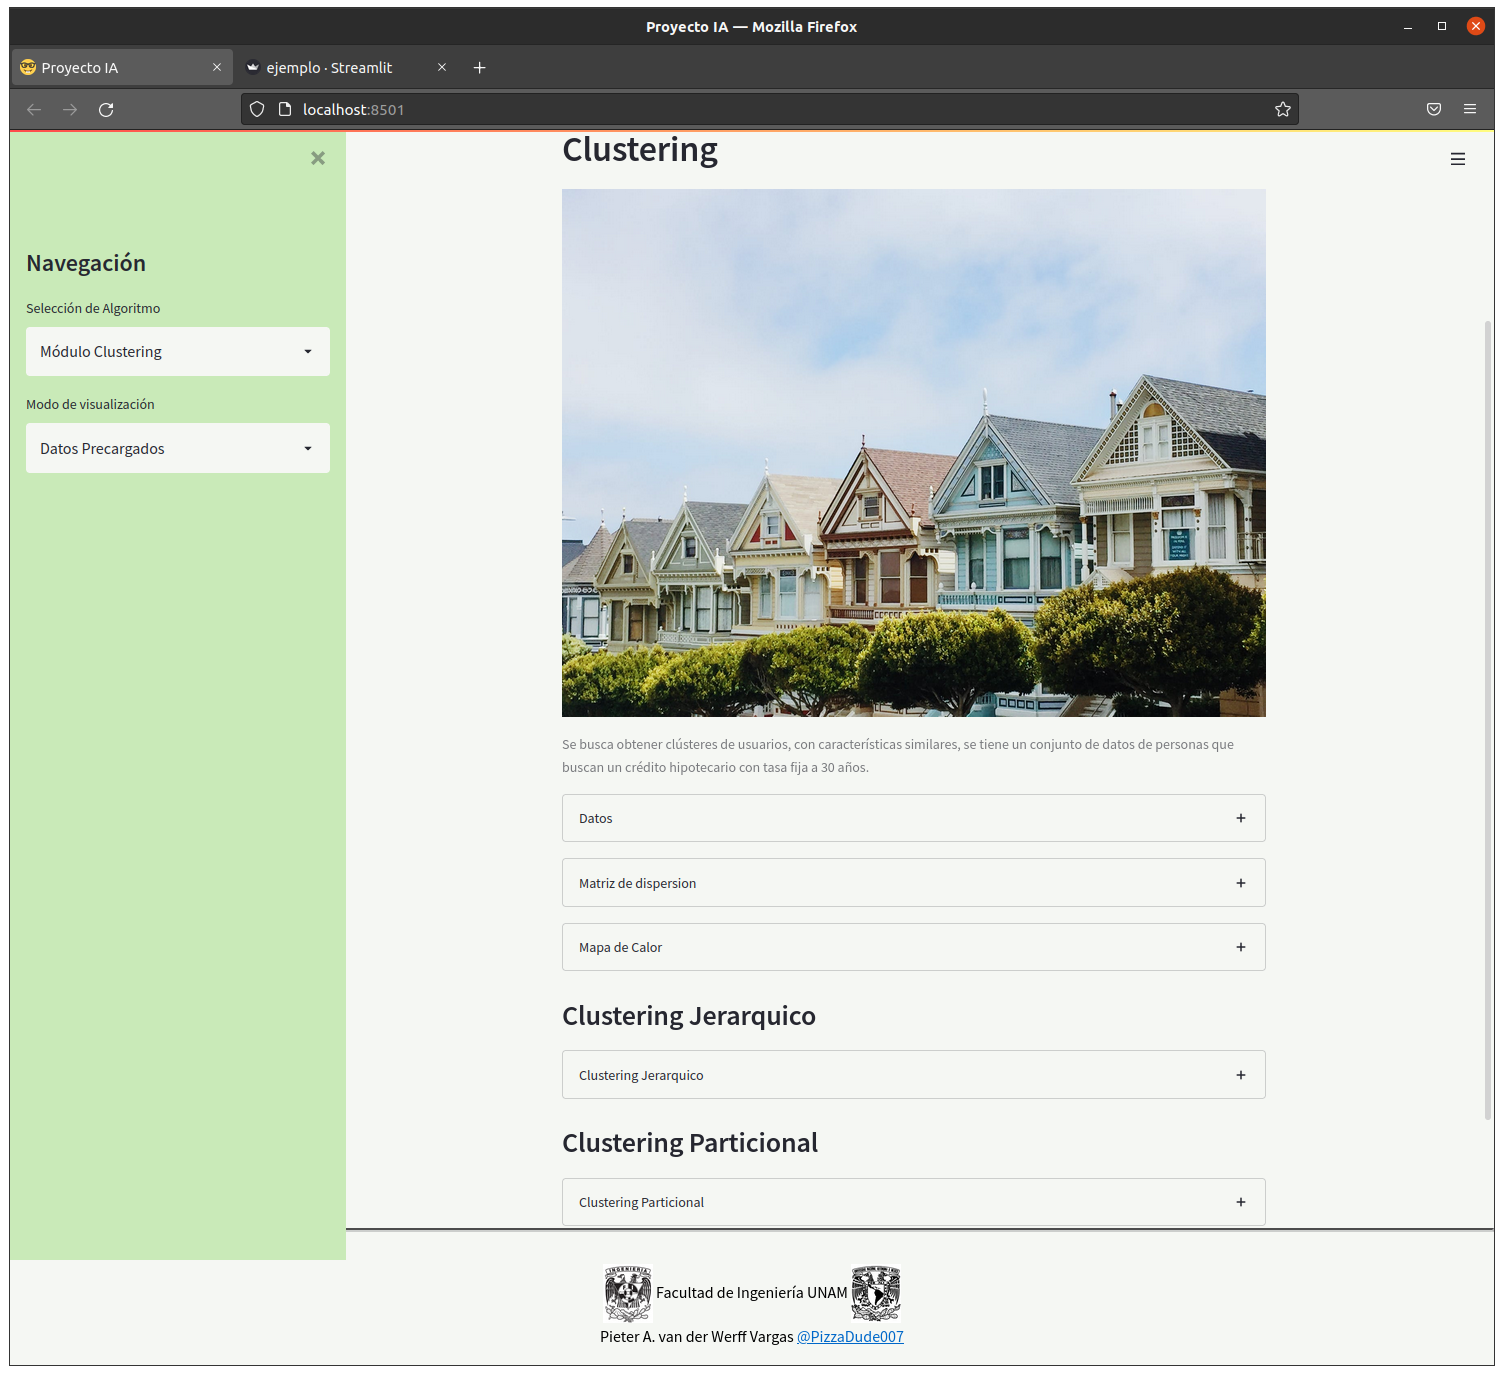
\includegraphics[height=6cm]{img/ClusteringDP_cerrado.png}
    \caption{Datos Precargados}
    \label{fig:ClusteringDP}
    \end{subfigure}
    \begin{subfigure}{0.5\textwidth}
    \centering
    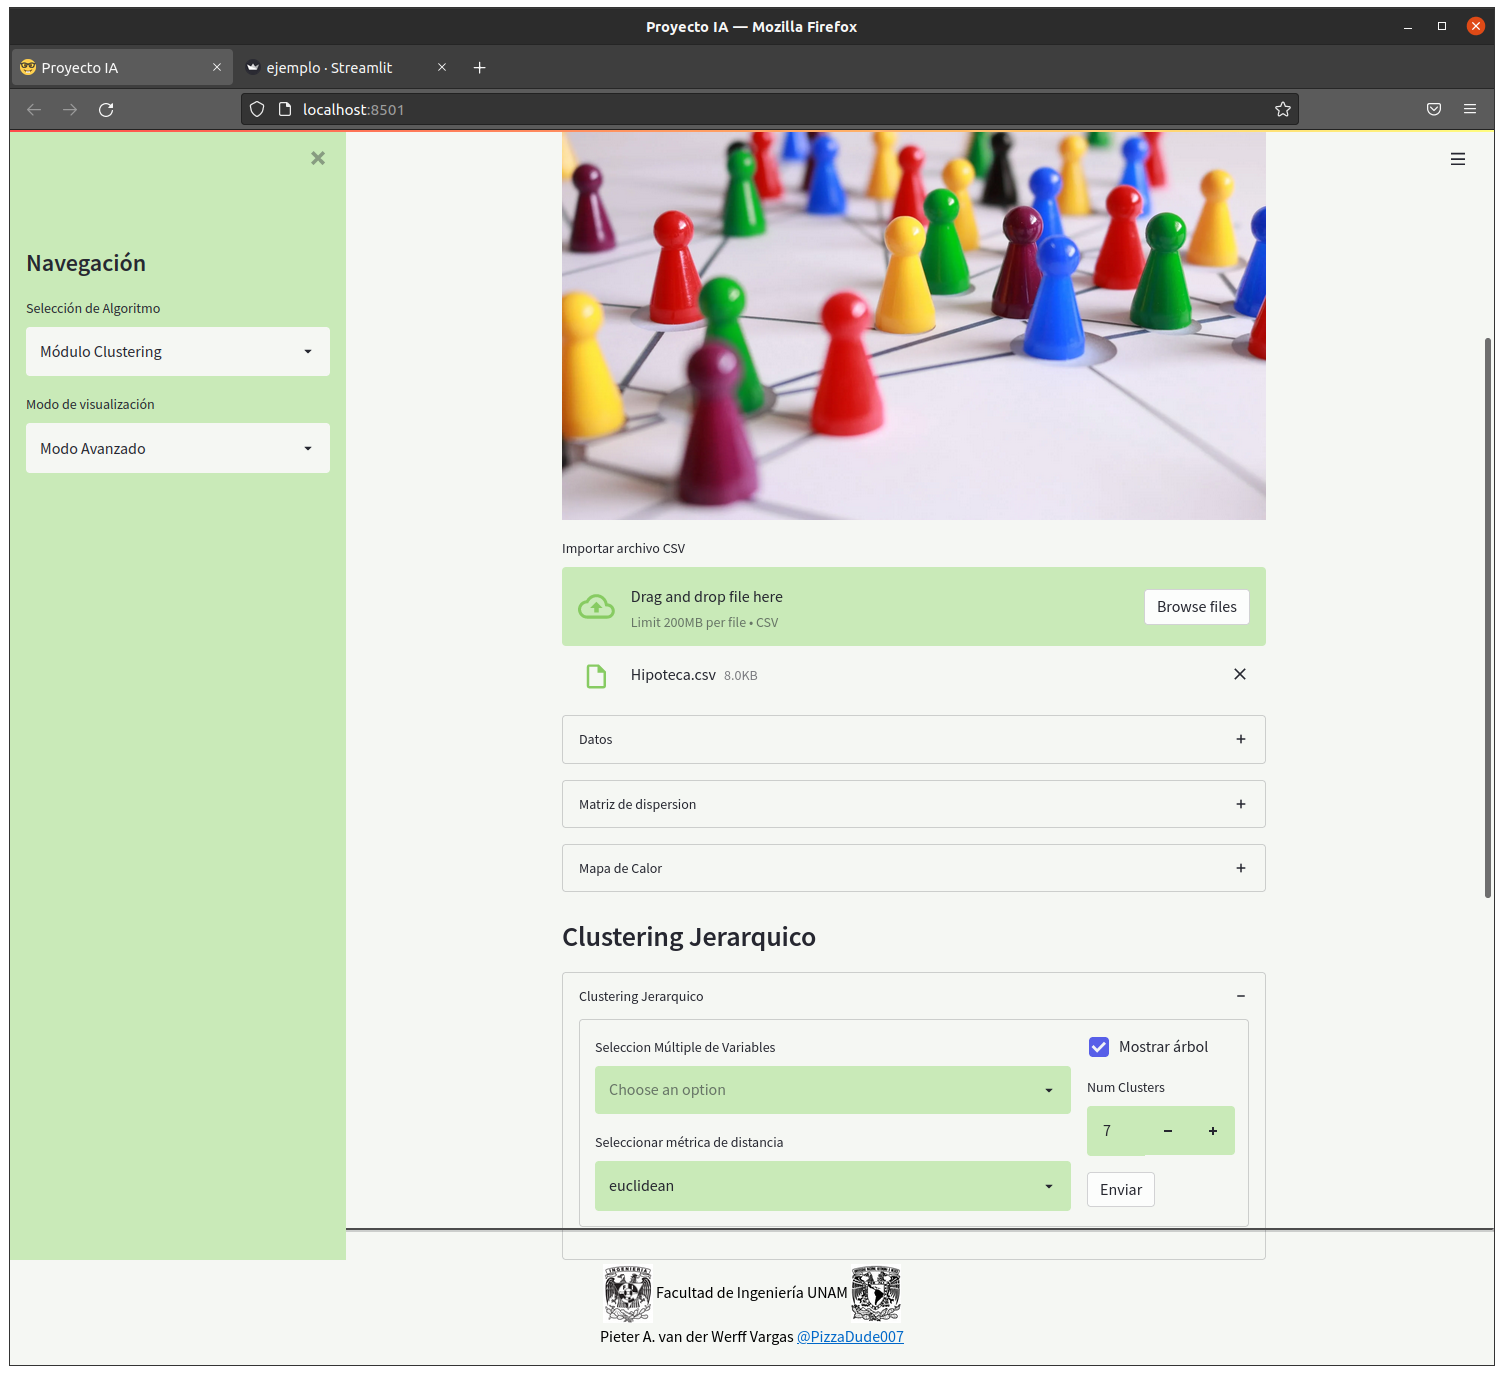
\includegraphics[height=6cm]{img/ClusteringMA.png}
    \caption{Modo Avanzado}
    \label{fig:ClusteringMA}
    \end{subfigure}
    
    \caption{Módulo Clustering}
    \label{fig:Clustering}
    \end{figure}
    
    Para el módulo de clustering se tienen dos algoritmos: el clustering jerárquico y el clustering particional. Si se utiliza el modo de visualización de tipo \textit{Datos Precargados} se utilizará un conjunto de datos de personas con características similares, que buscan un crédito hipotecario con una tasa fija a 30 años. Independientemente del modo de visualización, se generará un mapa de calor para una matriz de correlación de los datos; así como una matriz de dispersión, la cual es posible "colorear" con alguna de las variables del conjunto de datos, de forma que se pueda observar las variables o columnas que tienen mayor correlación, para elegir con cuáles trabajar el algoritmo.\newline

    \begin{figure}[H]
    
    \begin{subfigure}{0.5\textwidth}
    \centering
    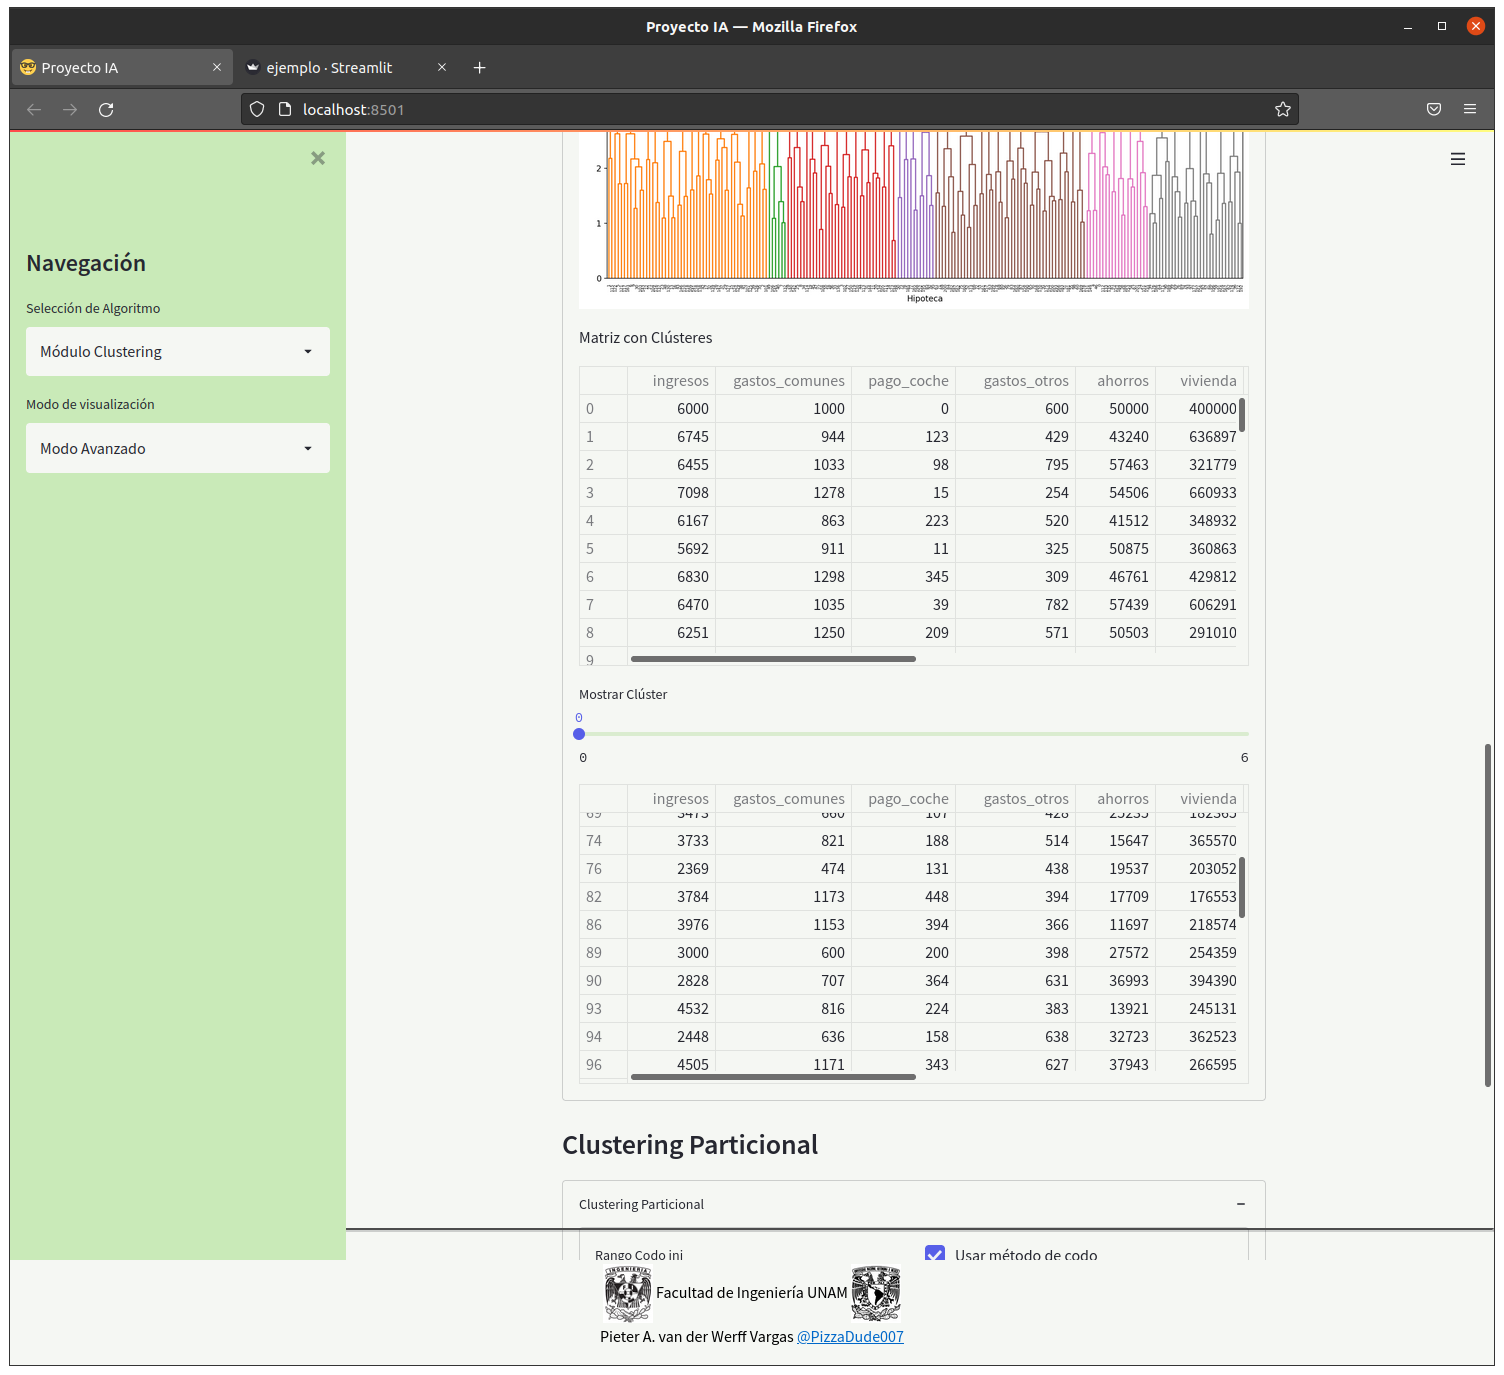
\includegraphics[height=6cm]{img/ClusteringMA_J.png} 
    \caption{Clustering Jerárquico}
    \label{fig:ClusteringJ}
    \end{subfigure}
    \begin{subfigure}{0.5\textwidth}
    \centering
    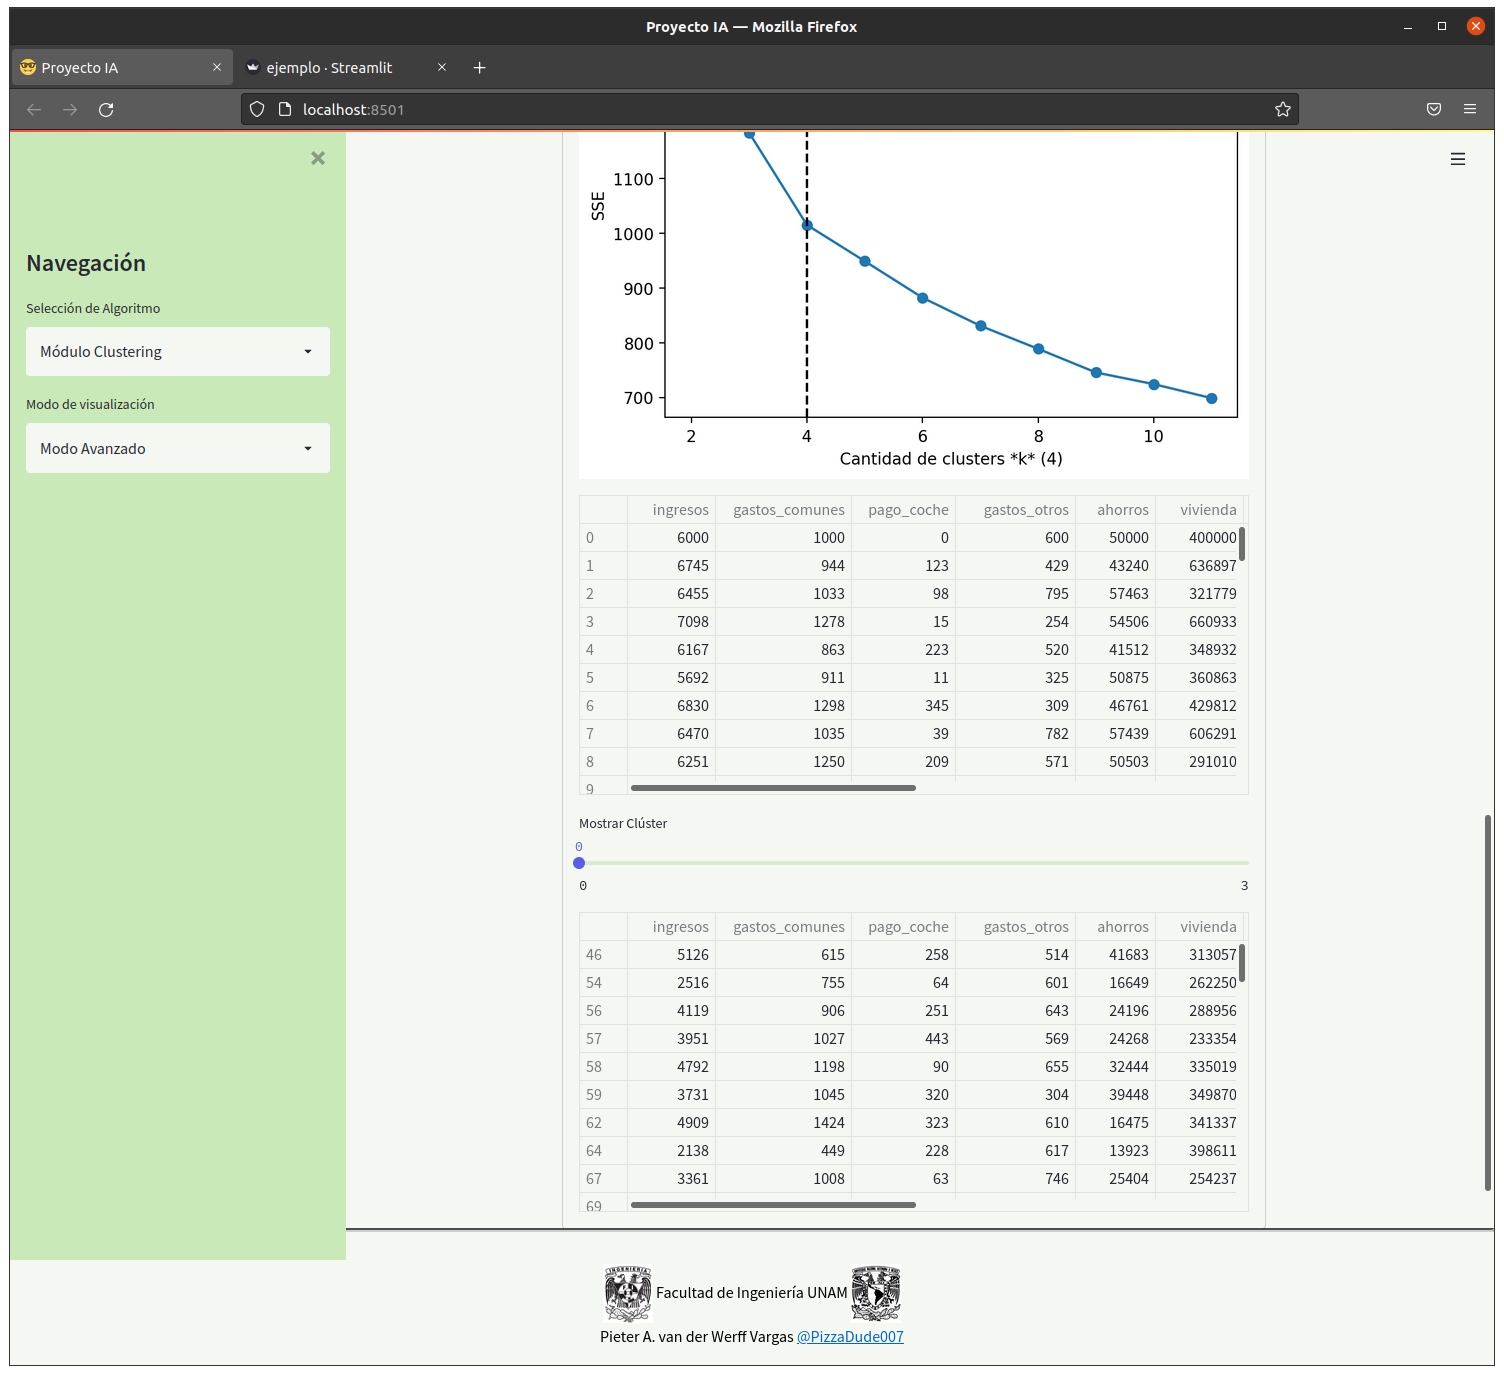
\includegraphics[height=6cm]{img/ClusteringMA_P.png}
    \caption{Clustering Particional}
    \label{fig:ClustringP}
    \end{subfigure}
    
    \caption{Salidas Clustering Modo Avanzado}
    \label{fig:ClusteringMA}
    \end{figure}
    
    \begin{figure}[H]
    
    \begin{subfigure}{0.5\textwidth}
    \centering
    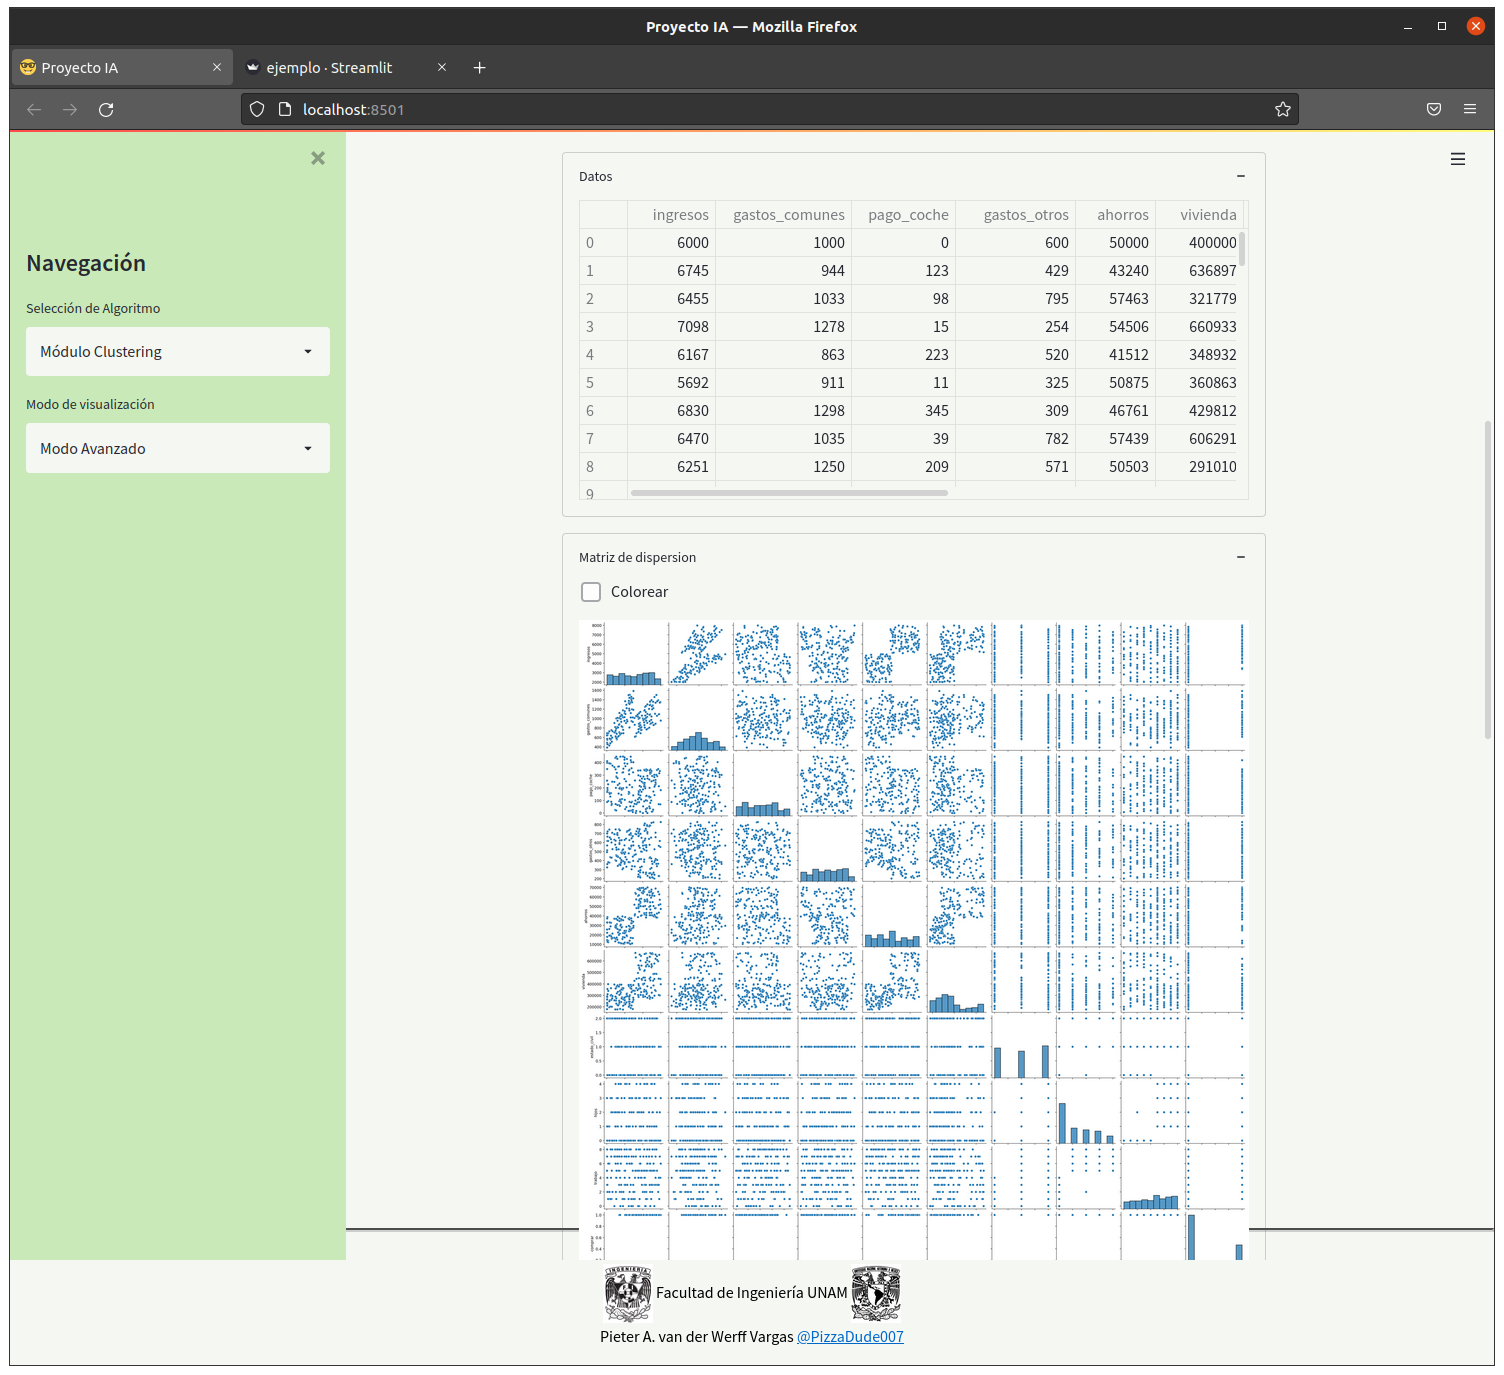
\includegraphics[height=6cm]{img/Clustering_dispersion.png} 
    \caption{Matriz de Dispersión}
    \label{fig:ClusteringDisp}
    \end{subfigure}
    \begin{subfigure}{0.5\textwidth}
    \centering
    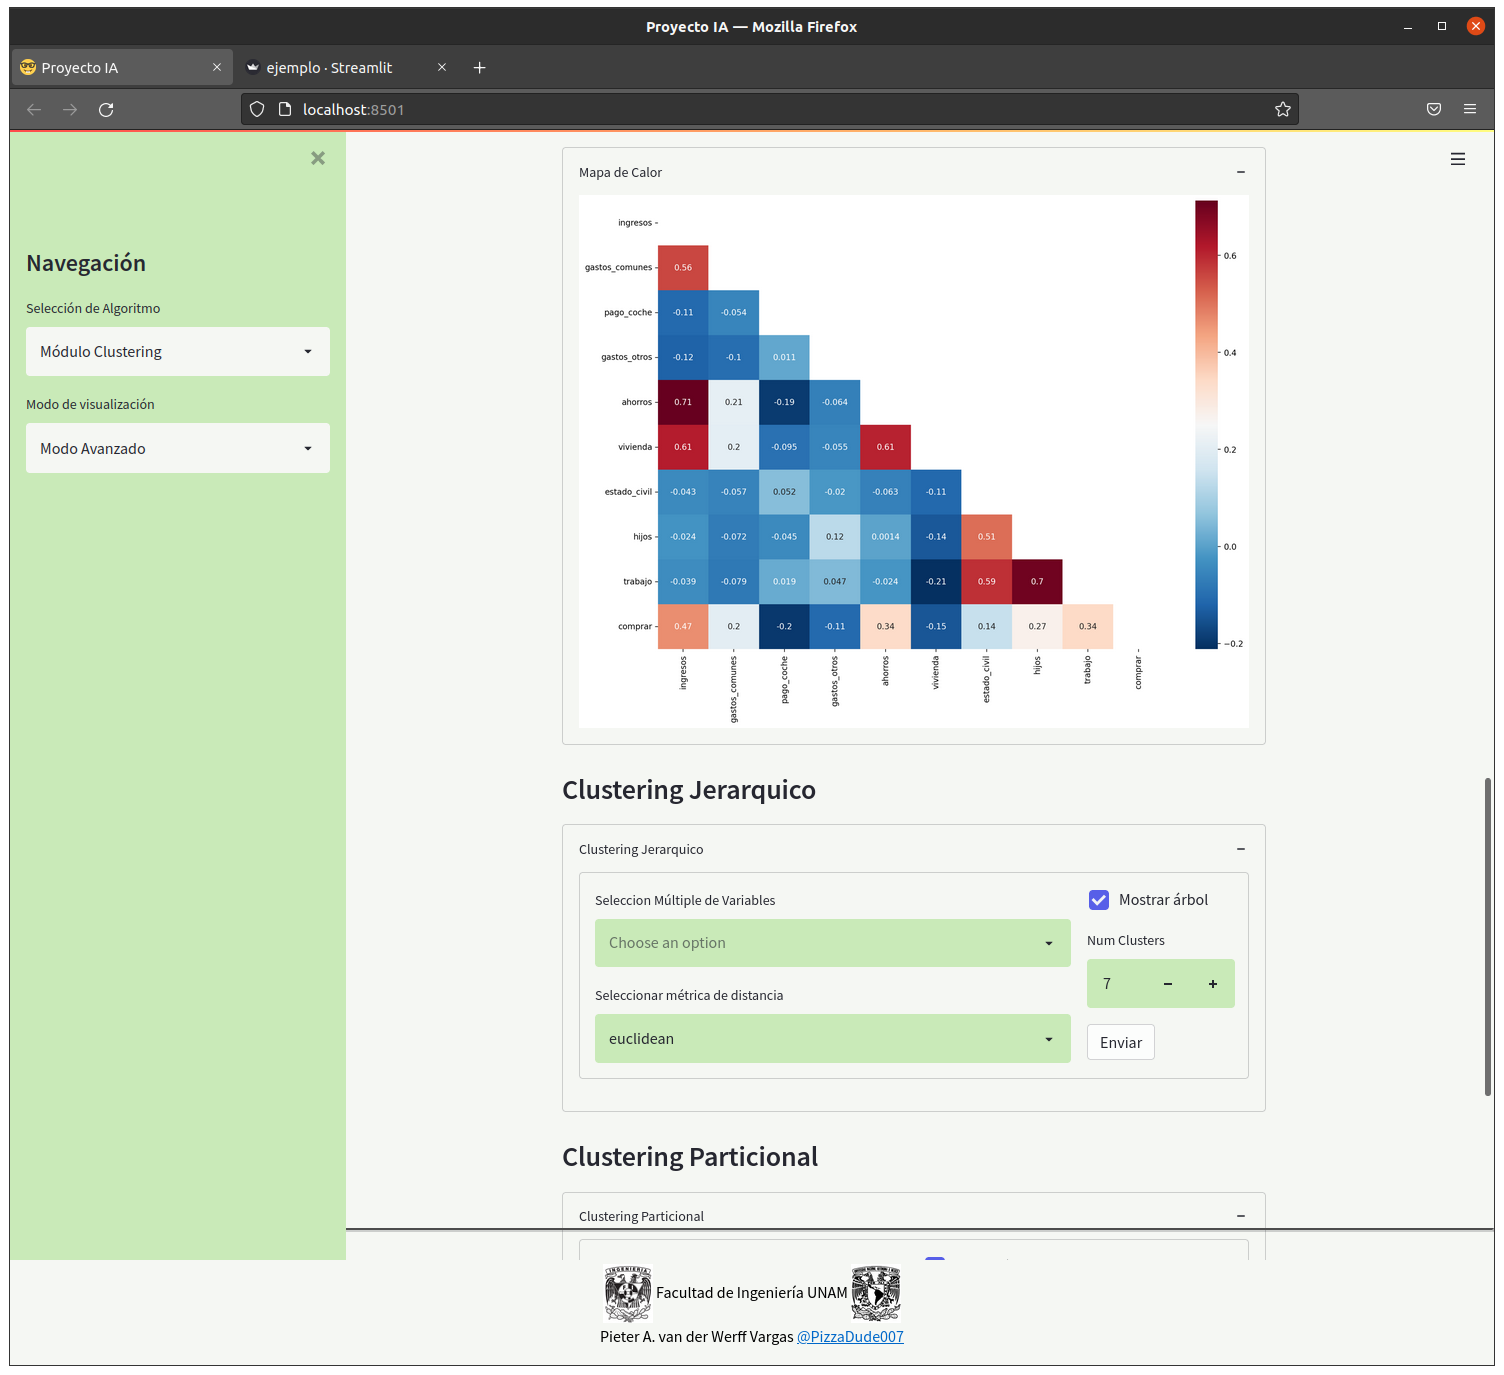
\includegraphics[height=6cm]{img/Clustering_HeatMap.png}
    \caption{Mapa de calor}
    \label{fig:ClustringHM}
    \end{subfigure}
    
    \caption{Matrices para evaluar variables}
    \label{fig:ClusteringDatos}
    \end{figure}
    
    Para este módulo, si se utiliza el modo de visualización de \textit{Datos Precargados} es posible realizar las mismas modificaciones a los parámetros de entrada del algoritmo que con el \textit{Modo Avanzado}, la única diferencia siendo que no es necesario seleccionar las variables y las gráficas para cada algoritmo se encuentran escondidas por default. En ambos casos es posible modificar para el algoritmo de Clustering Jerárquico, el tipo de métrica de distancia y número de clústeres; así como elegir si se quiere utilizar el método del codo o una cantidad especifica de clústeres para el algoritmo de k-means (Clustering Particional).
    
\subsection{Clasificación Regresión Logística}

    \begin{figure}[H]
    
    \begin{subfigure}{0.5\textwidth}
    \centering
    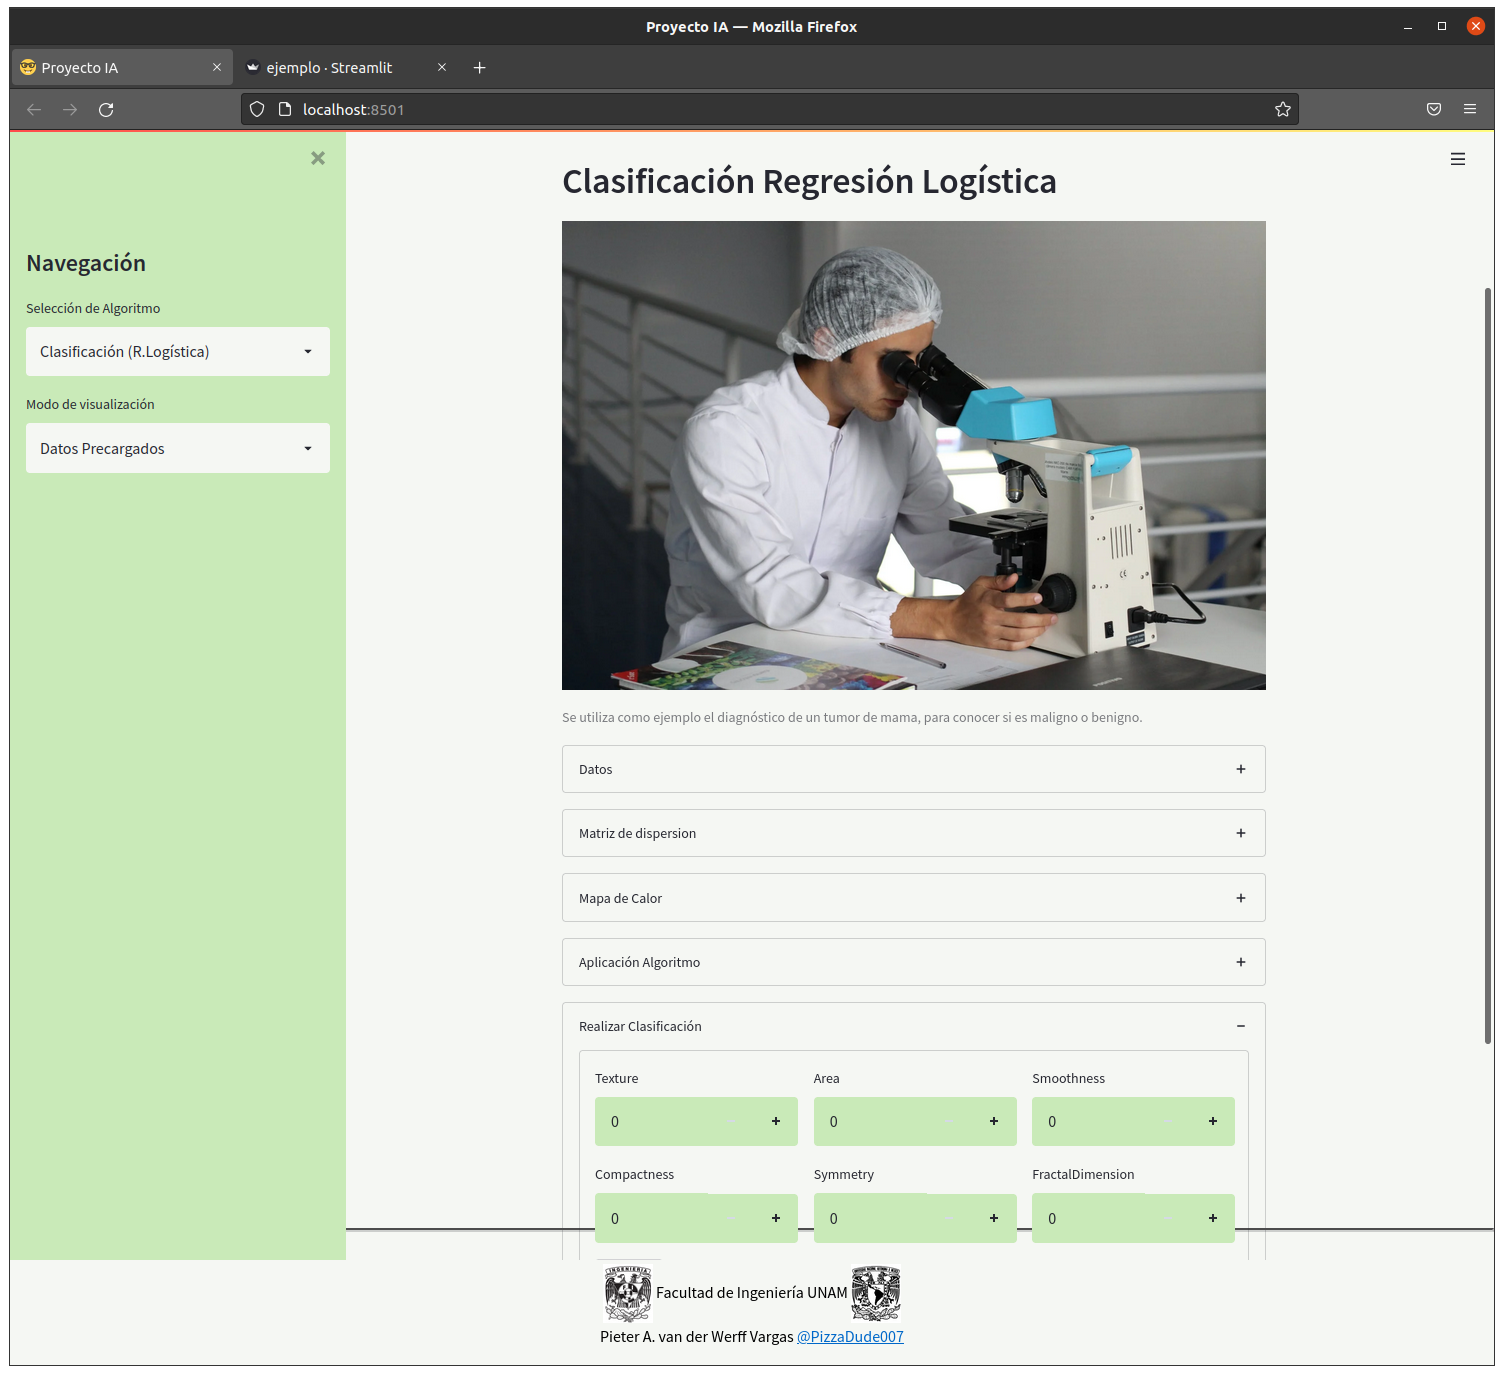
\includegraphics[height=6cm]{img/RLogisticaDP.png} 
    \caption{Datos Precargados}
    \label{fig:RLDP}
    \end{subfigure}
    \begin{subfigure}{0.5\textwidth}
    \centering
    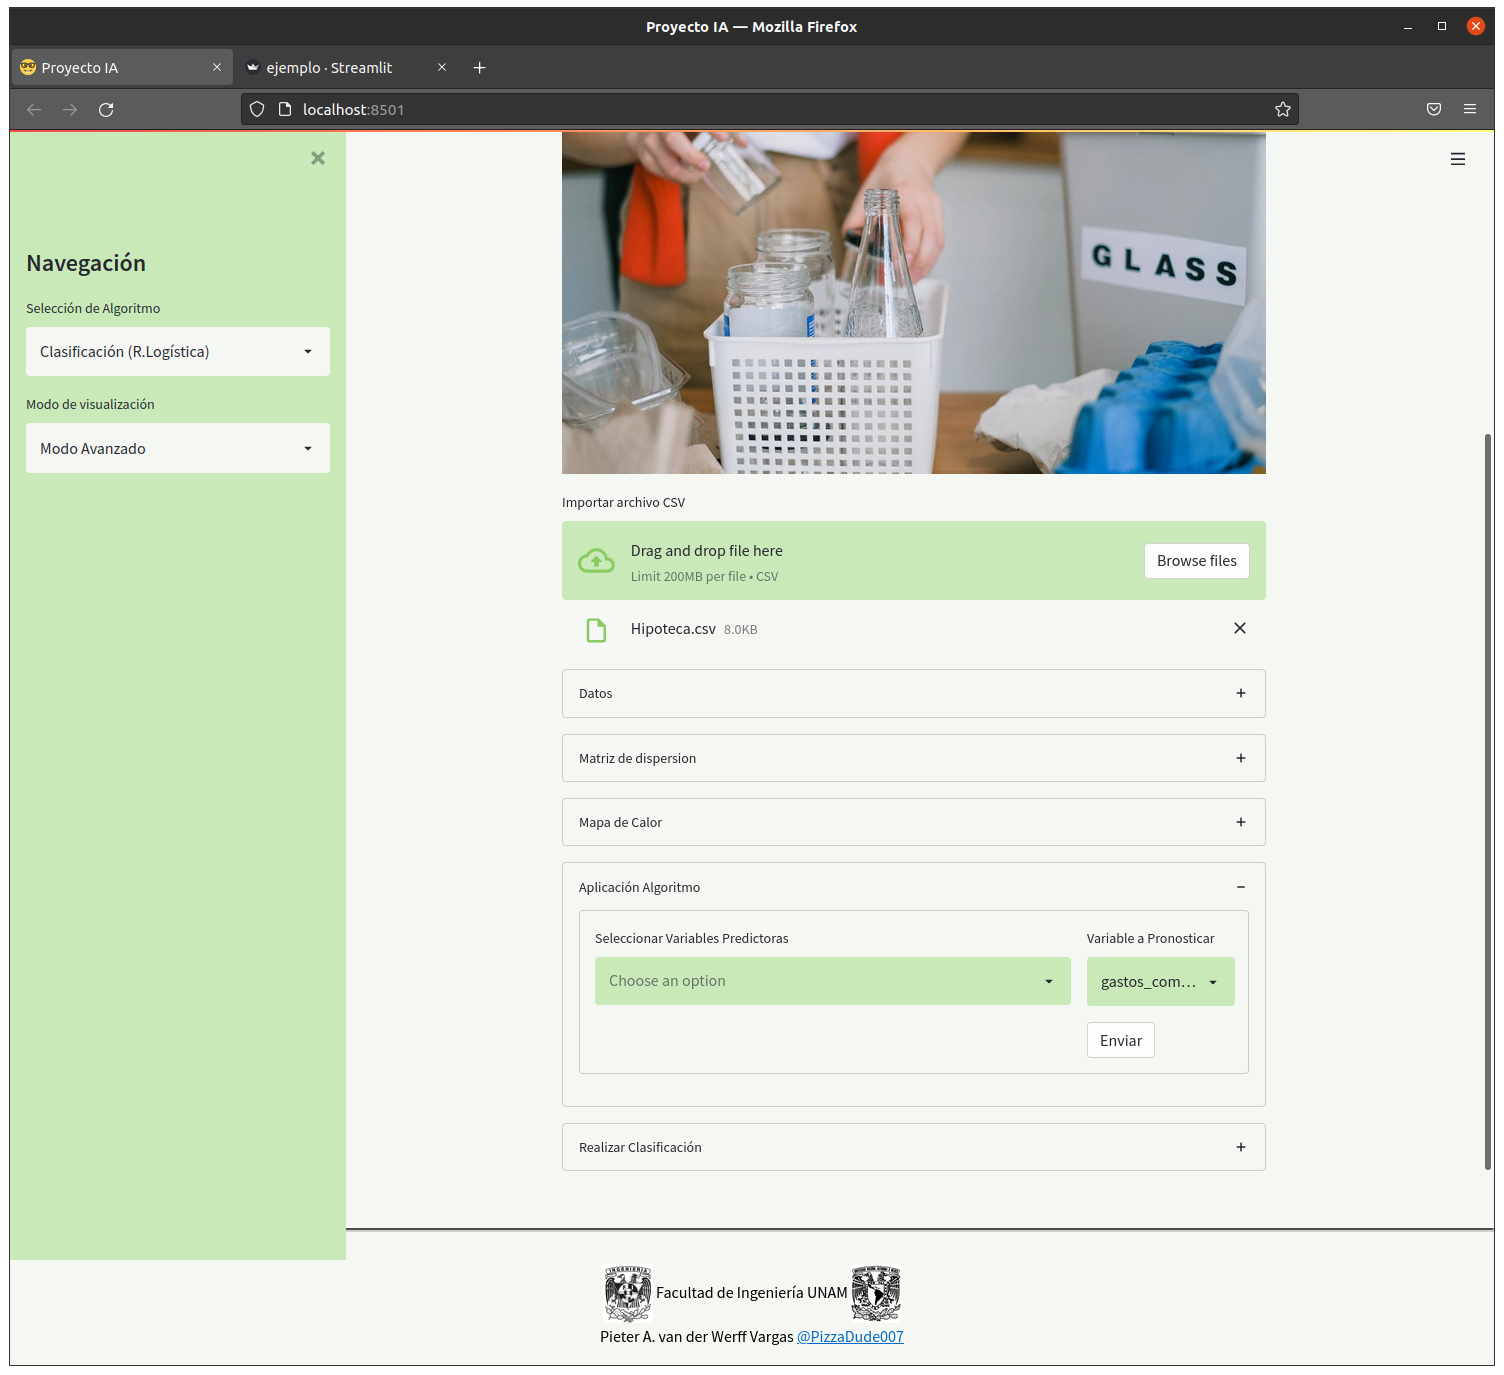
\includegraphics[height=6cm]{img/RLogisticaMA.png}
    \caption{Modo Avanzado}
    \label{fig:RLMA}
    \end{subfigure}
    
    \caption{Regresión Logística}
    \label{fig:RLogistic}
    \end{figure}
    
    Para este algoritmo, la diferencia entre los parámetros que contiene la visualización del modo \textit{Datos Precargados} y \textit{Modo Avanzado} es más notable. Comenzando con lo que tienen en común ambos modos de visualización, es posible observar primeramente una matriz de dispersión, la cuál es posible "colorear" respecto a la carga de una de nuestras variables. Además, podemos visualizar una matriz de correlación en la cual se tiene un mapa de calor para observar cuales variables nos son útiles al cargar los datos en nuestro modelo. Estas características se muestran en la figura siguiente.
    
    \begin{figure}[H]
    
    \begin{subfigure}{0.5\textwidth}
    \centering
    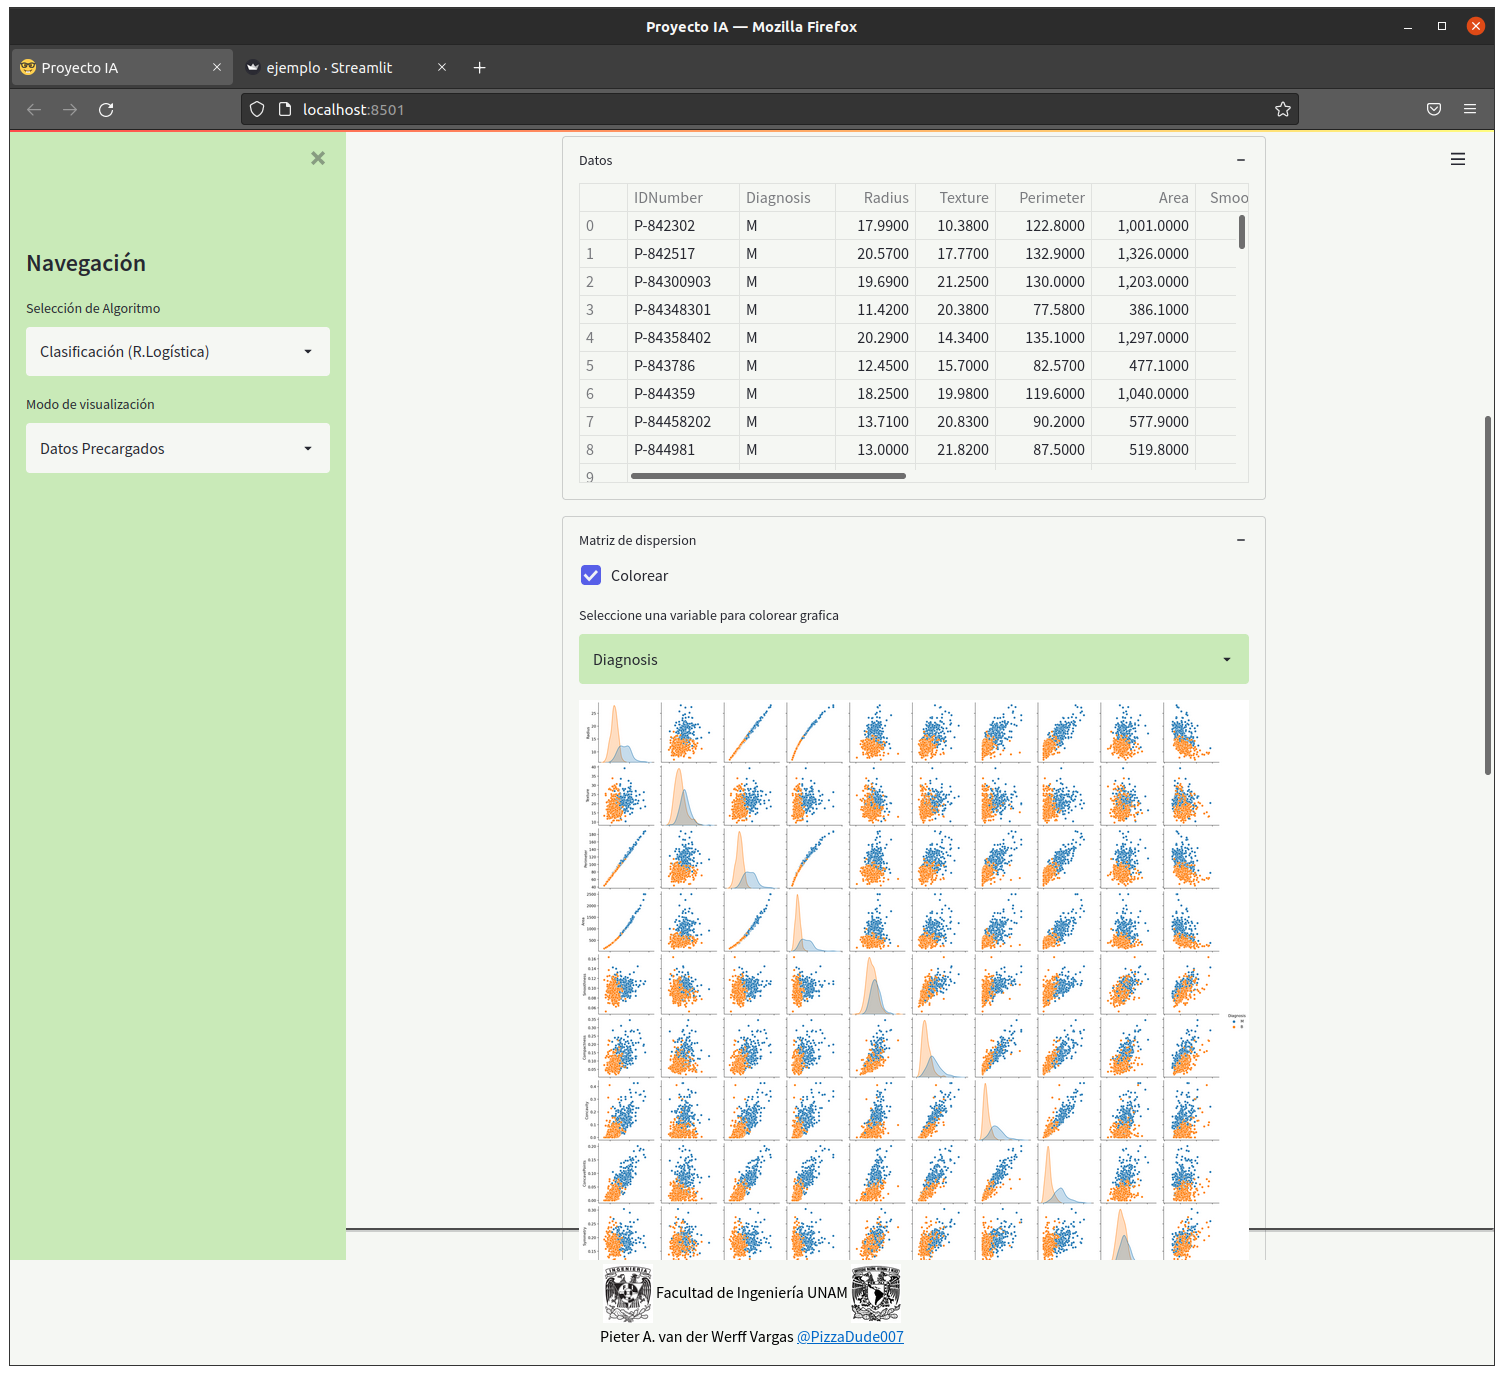
\includegraphics[height=6cm]{img/RLogistica_MDispersion.png} 
    \caption{Matriz de Dispersión}
    \label{fig:RLMD}
    \end{subfigure}
    \begin{subfigure}{0.5\textwidth}
    \centering
    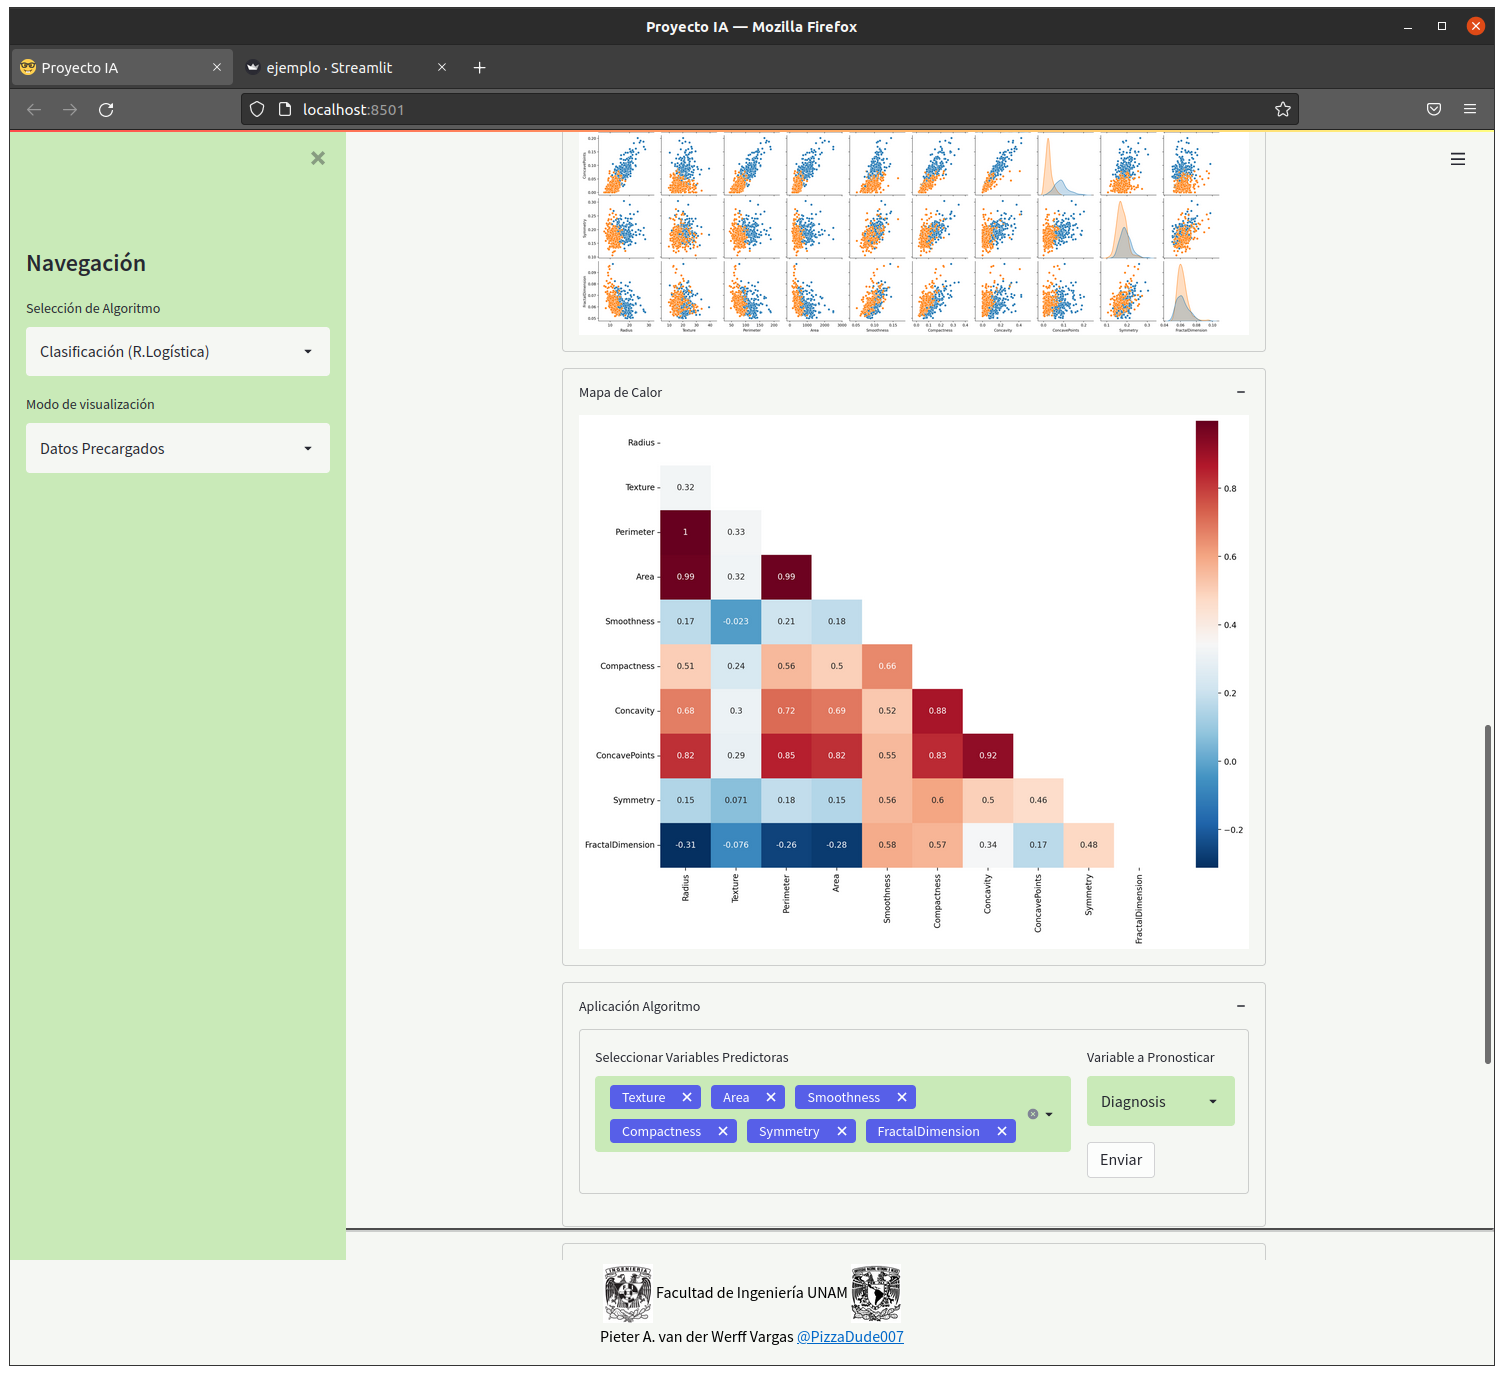
\includegraphics[height=6cm]{img/RLogistica_HeatMap.png}
    \caption{Mapa de Calor}
    \label{fig:RLHM}
    \end{subfigure}
    
    \caption{Visualización de matrices}
    \label{fig:RLogisticVar}
    \end{figure}
    
    Para la visualización de tipo \textit{Datos Precargados} se puede únicamente modificar los parámetros de entrada de nuestro conjunto de datos de una población de personas pacientes para diagnosticar si su tumor de mama es de tipo benigno o maligno, para obtener un diagnóstico directamente. Por otra parte, si se utiliza el modo de visualización de \textit{Modo Avanzado} es posible modificar adicionalmente los parámetros del tamaño de muestra y la semilla que se utiliza para la generación aleatoria de esta. Adicionalmente en este modo, se observa distintas matrices para evaluar su eficiencia, así como el porcentaje de exactitud del algoritmo y observar de mejor manera si su predicción es correcta así como el funcionamiento de este algoritmo.
    
    \begin{figure}[H]
    
    \begin{subfigure}{0.5\textwidth}
    \centering
    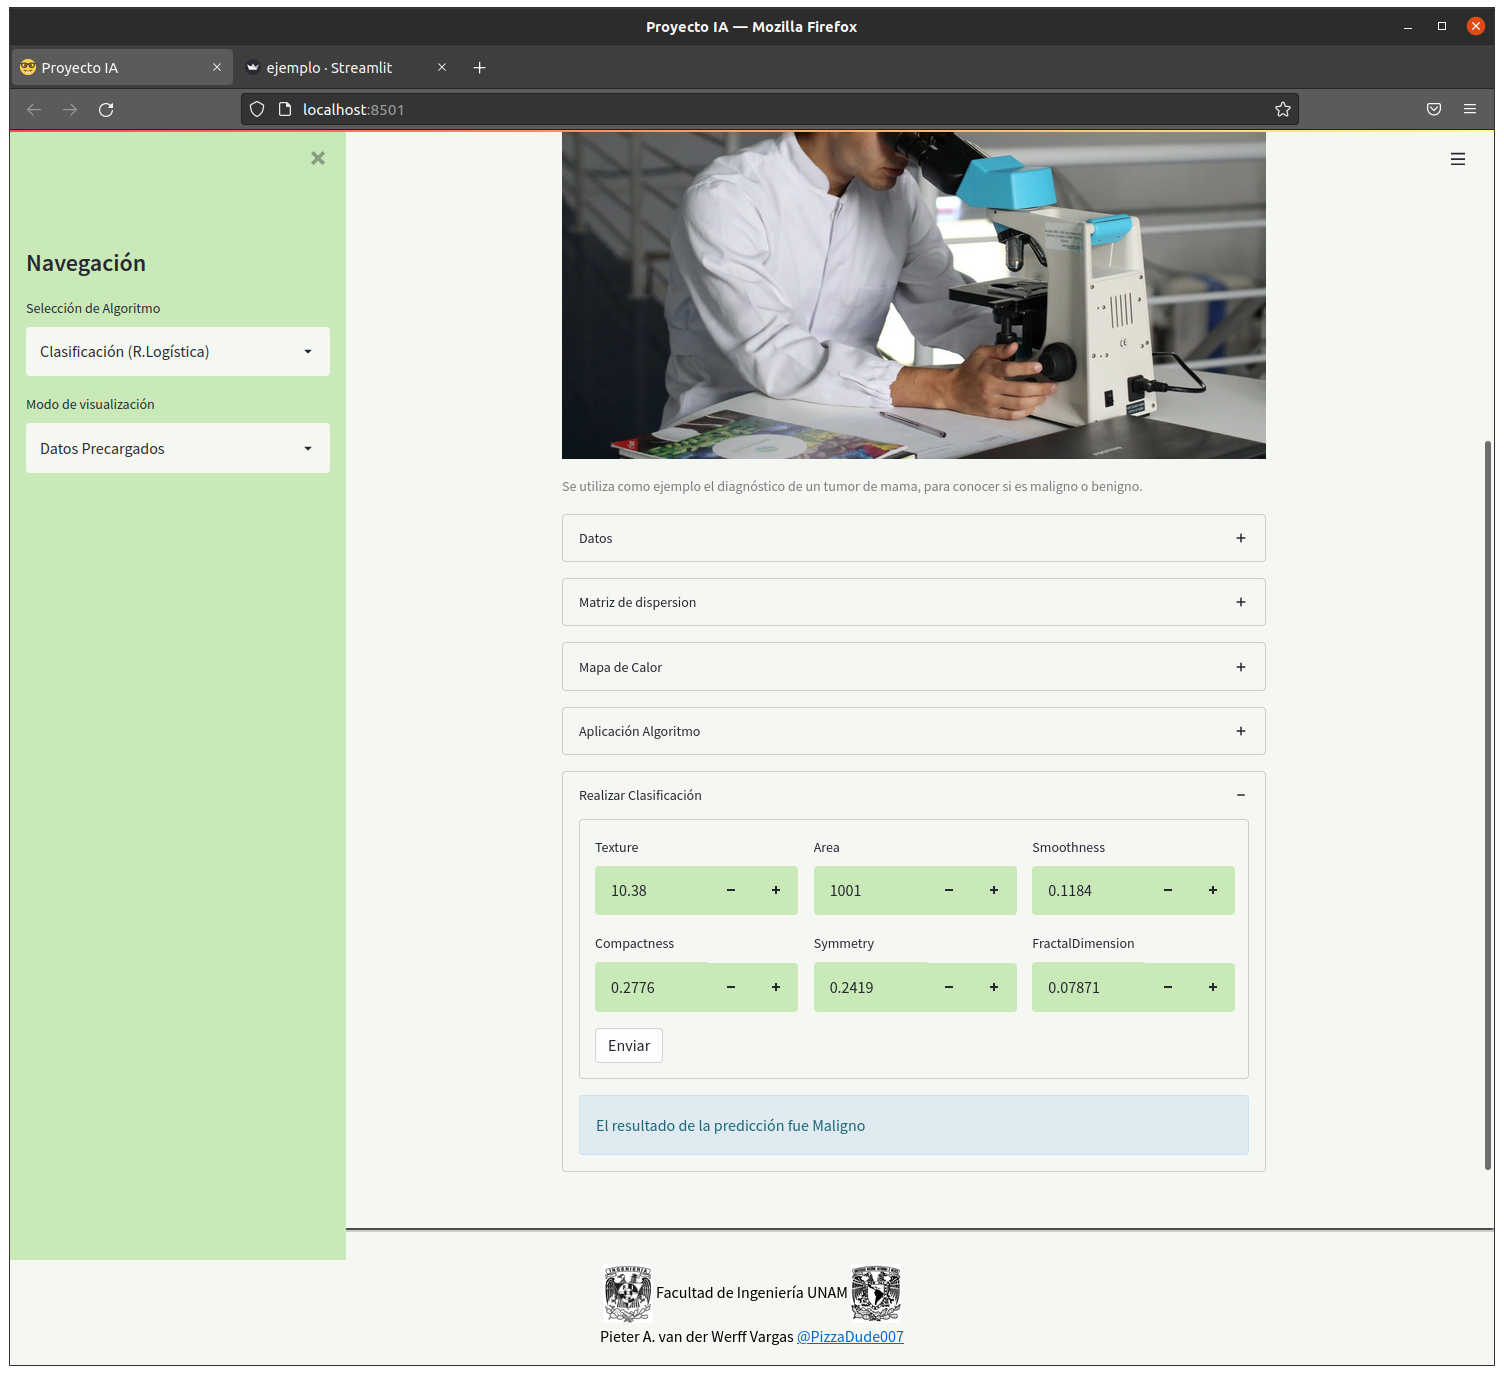
\includegraphics[height=6cm]{img/RLogisticaDP_resultados.png} 
    \caption{Salida Datos Precargados}
    \label{fig:RLDPres}
    \end{subfigure}
    \begin{subfigure}{0.5\textwidth}
    \centering
    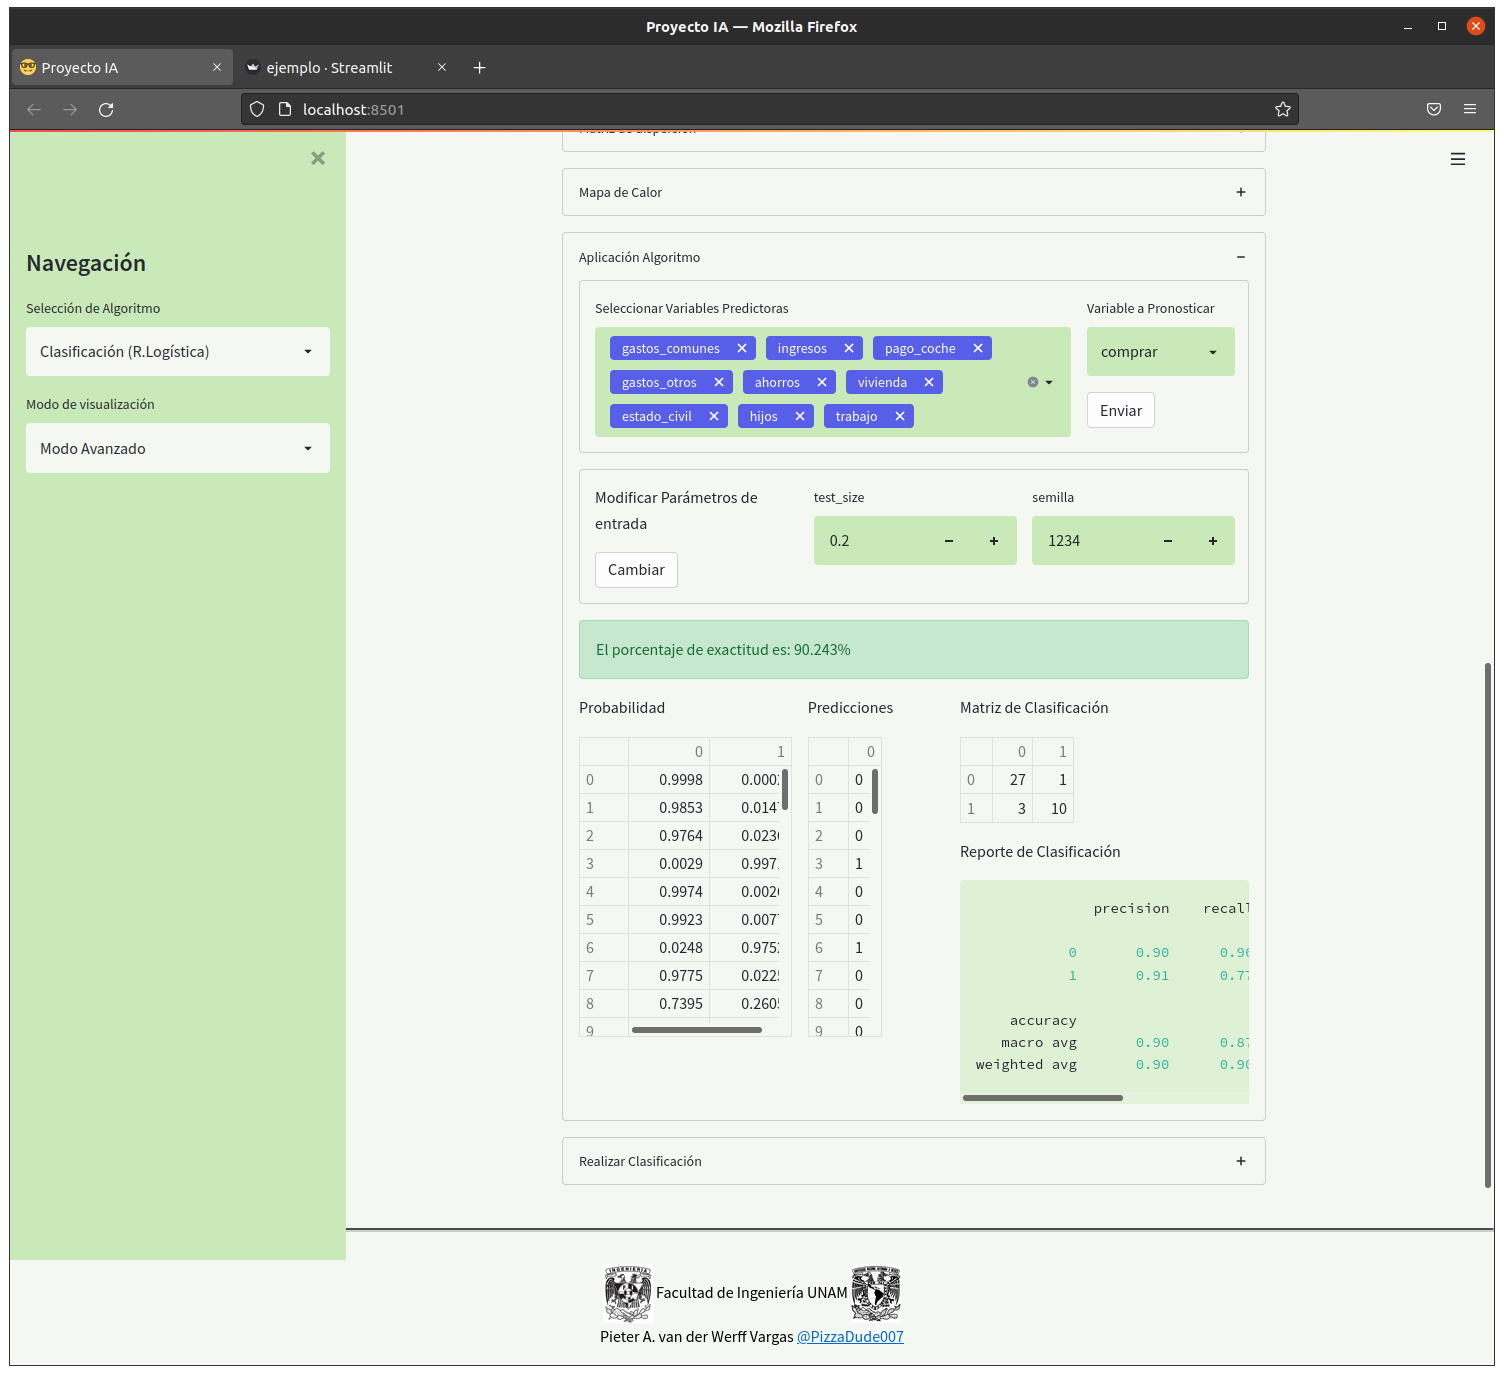
\includegraphics[height=6cm]{img/RLogisticaMA_resultados.png}
    \caption{Parámetros Modo Avanzado}
    \label{fig:RLMAres}
    \end{subfigure}
    
    \caption{Resultados Clasificación Regresión Logística}
    \label{fig:RLogisticRes}
    \end{figure}

\subsection{Módulo Árboles}

    \begin{figure}[H]
    
    \begin{subfigure}{0.5\textwidth}
    \centering
    \includegraphics[height=6cm]{img/ÁrbolesDP.png} 
    \caption{Datos Precargados}
    \label{fig:ArbolDP}
    \end{subfigure}
    \begin{subfigure}{0.5\textwidth}
    \centering
    \includegraphics[height=6cm]{img/ÁrbolesMA.png}
    \caption{Modo Avanzado}
    \label{fig:ArbolMA}
    \end{subfigure}
    
    \caption{Modulo Árboles}
    \label{fig:Arboles}
    \end{figure}
    
    Este módulo incorpora dos algoritmos, el primero siendo árboles de regresión para realizar pronósticos y el segundo árboles de clasificación. En este módulo se tiene una gran diferenciación entre el modo de visualización de tipo \textit{Datos Precargados} y \textit{Modo Avanzado}, en este primero e utiliza un conjunto de datos para pacientes de un diagnóstico de tumor de mama. Se puede realizar un diagnóstico de si el tumor es benigno o maligno, de acuerdo con distintos parámetros en caso de utilizar el algoritmo de clasificación, de manera similar al funcionamiento en \ref{Clasificación Regresión Logística}. En el caso de la implementación de pronóstico se realiza, utilizando los mismos datos, una inferencia del tamaño de área que podría tener un tumor de mama, de acuerdo a ciertos parámetros.
    
    \begin{figure}[H]
    
    \begin{subfigure}{0.5\textwidth}
    \centering
    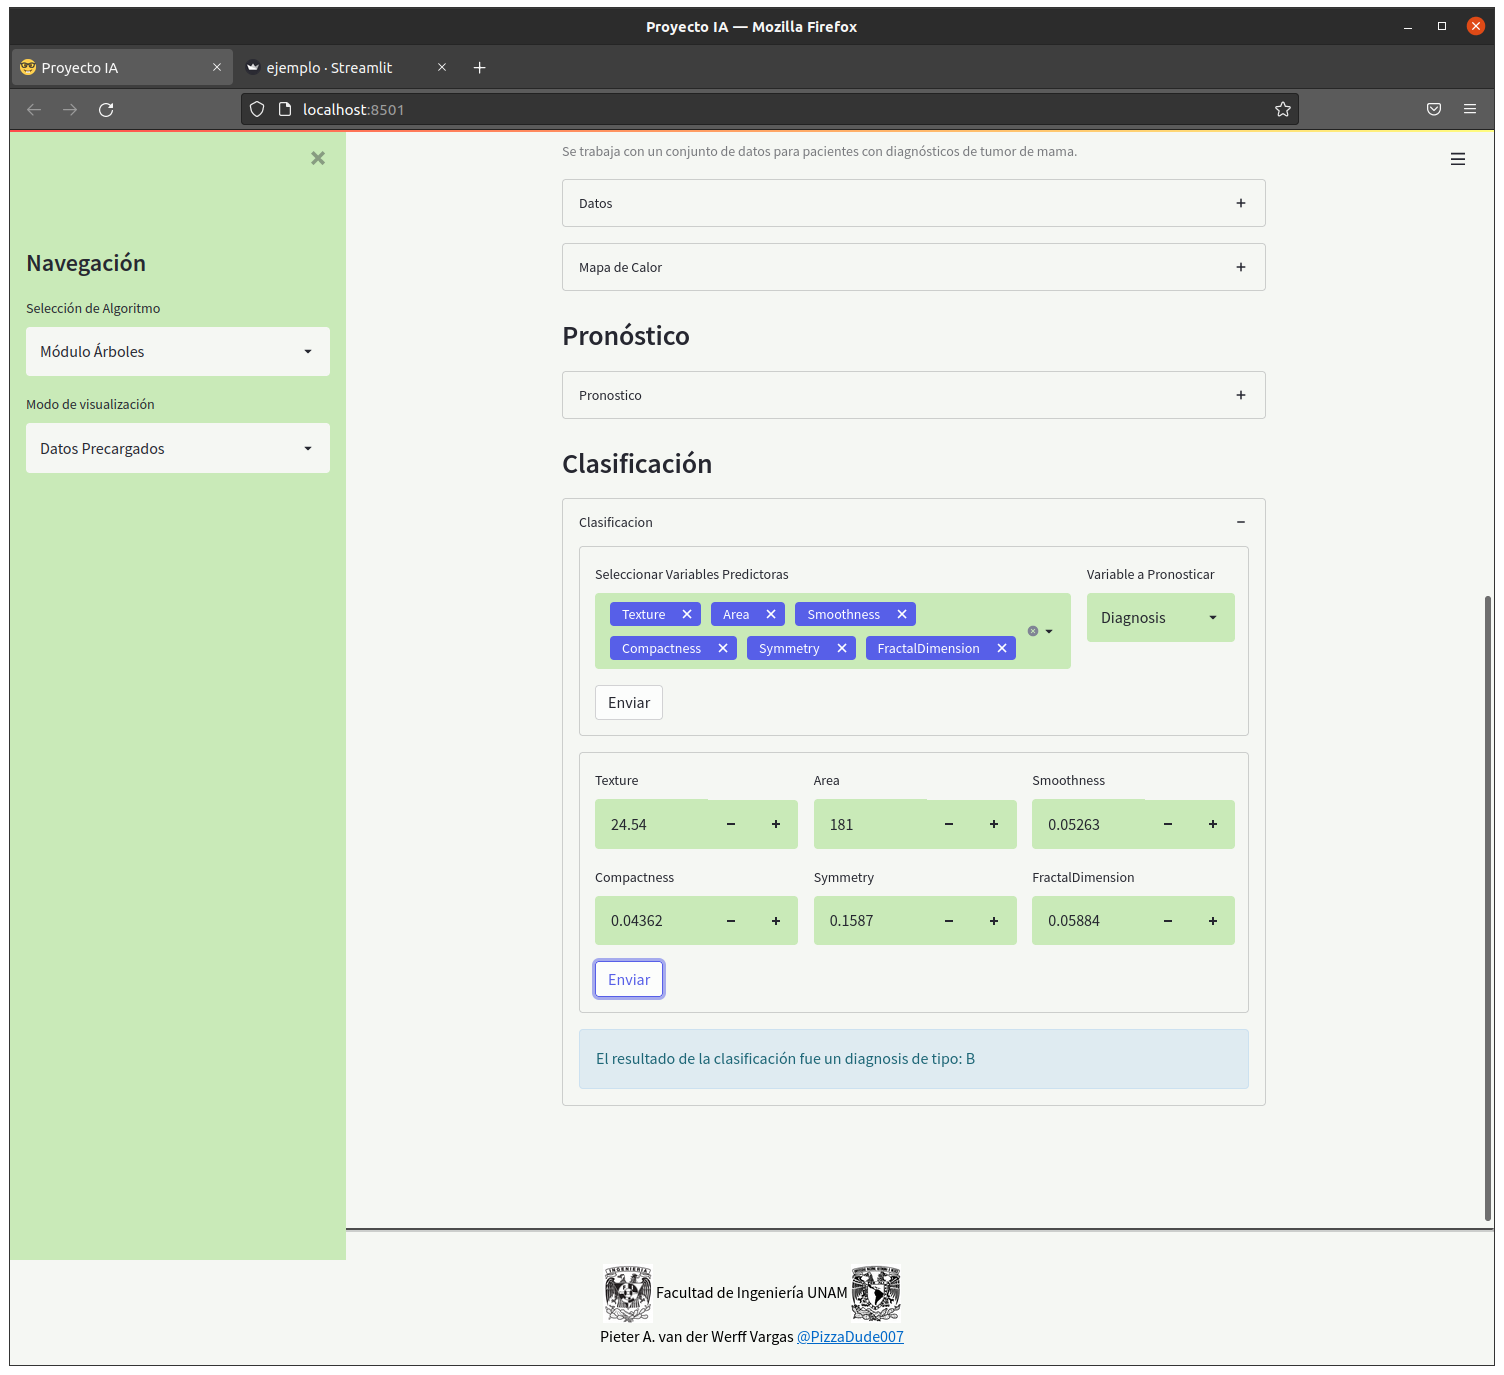
\includegraphics[height=6cm]{img/ÁrbolesClasificaciónDP.png} 
    \caption{Clasificación}
    \label{fig:ArbolDPc}
    \end{subfigure}
    \begin{subfigure}{0.5\textwidth}
    \centering
    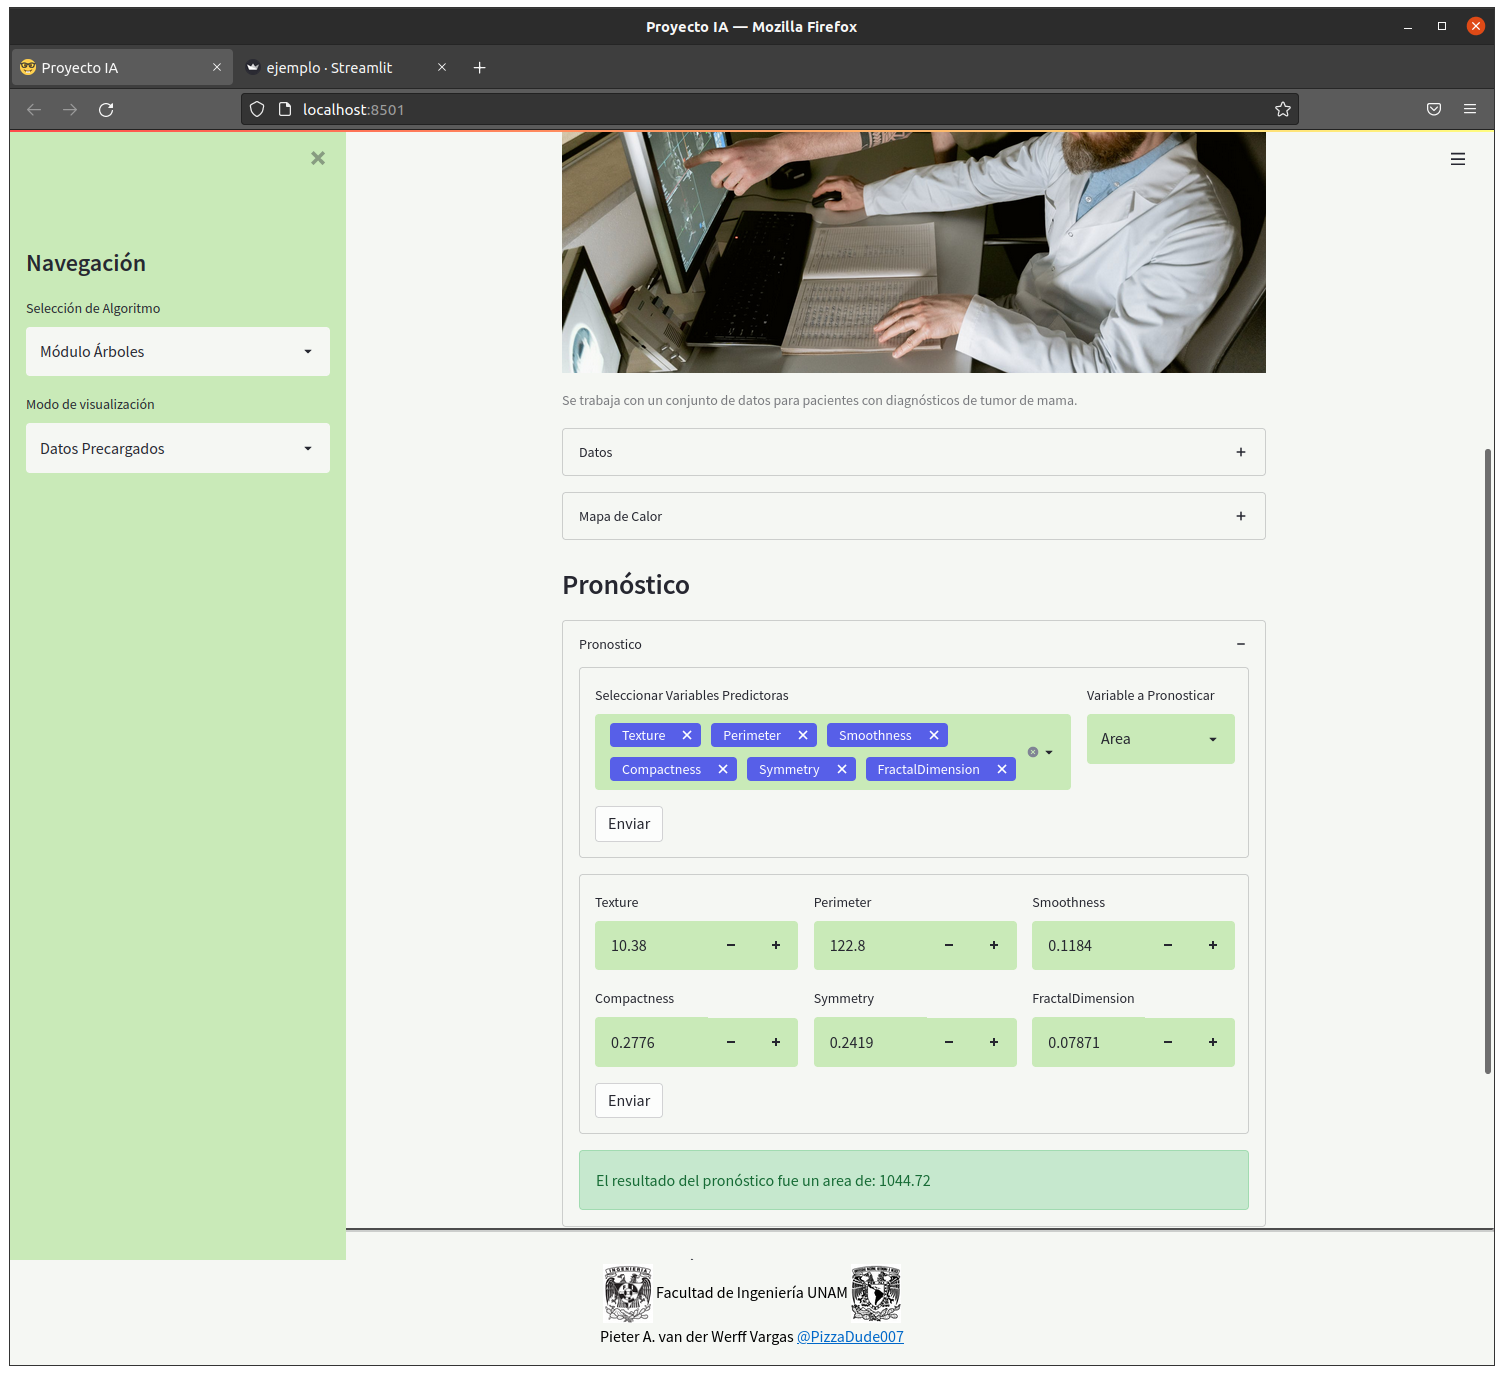
\includegraphics[height=6cm]{img/ÁrbolesPronósticoDP.png}
    \caption{Pronóstico}
    \label{fig:ArbolDPp}
    \end{subfigure}
    
    \caption{Ejecución Algoritmos (Datos Precargados)}
    \label{fig:ArbolesTDP}
    \end{figure}
    
    \begin{figure}[H]
    \centering
    \includegraphics[height=6cm]{img/Árboles_HeatMap.png} 
    \caption{Mapa de calor}
    \label{fig:ArbolHM}
    \end{figure}
    
    Independientemente del modo de visualización que se utilice, en ambos se puede visualizar una matriz de correlación, que utiliza un mapa de calor para visualizar que tanto nivel de correlación se tiene entre dos variables, de forma que se pueda descartar a aquellas que se acerquen a la unidad y se utilicen solo las variables que sean de utilidad para servir como variables predictoras en su respectivo algoritmo.
    
    \begin{figure}[H]
    \centering
    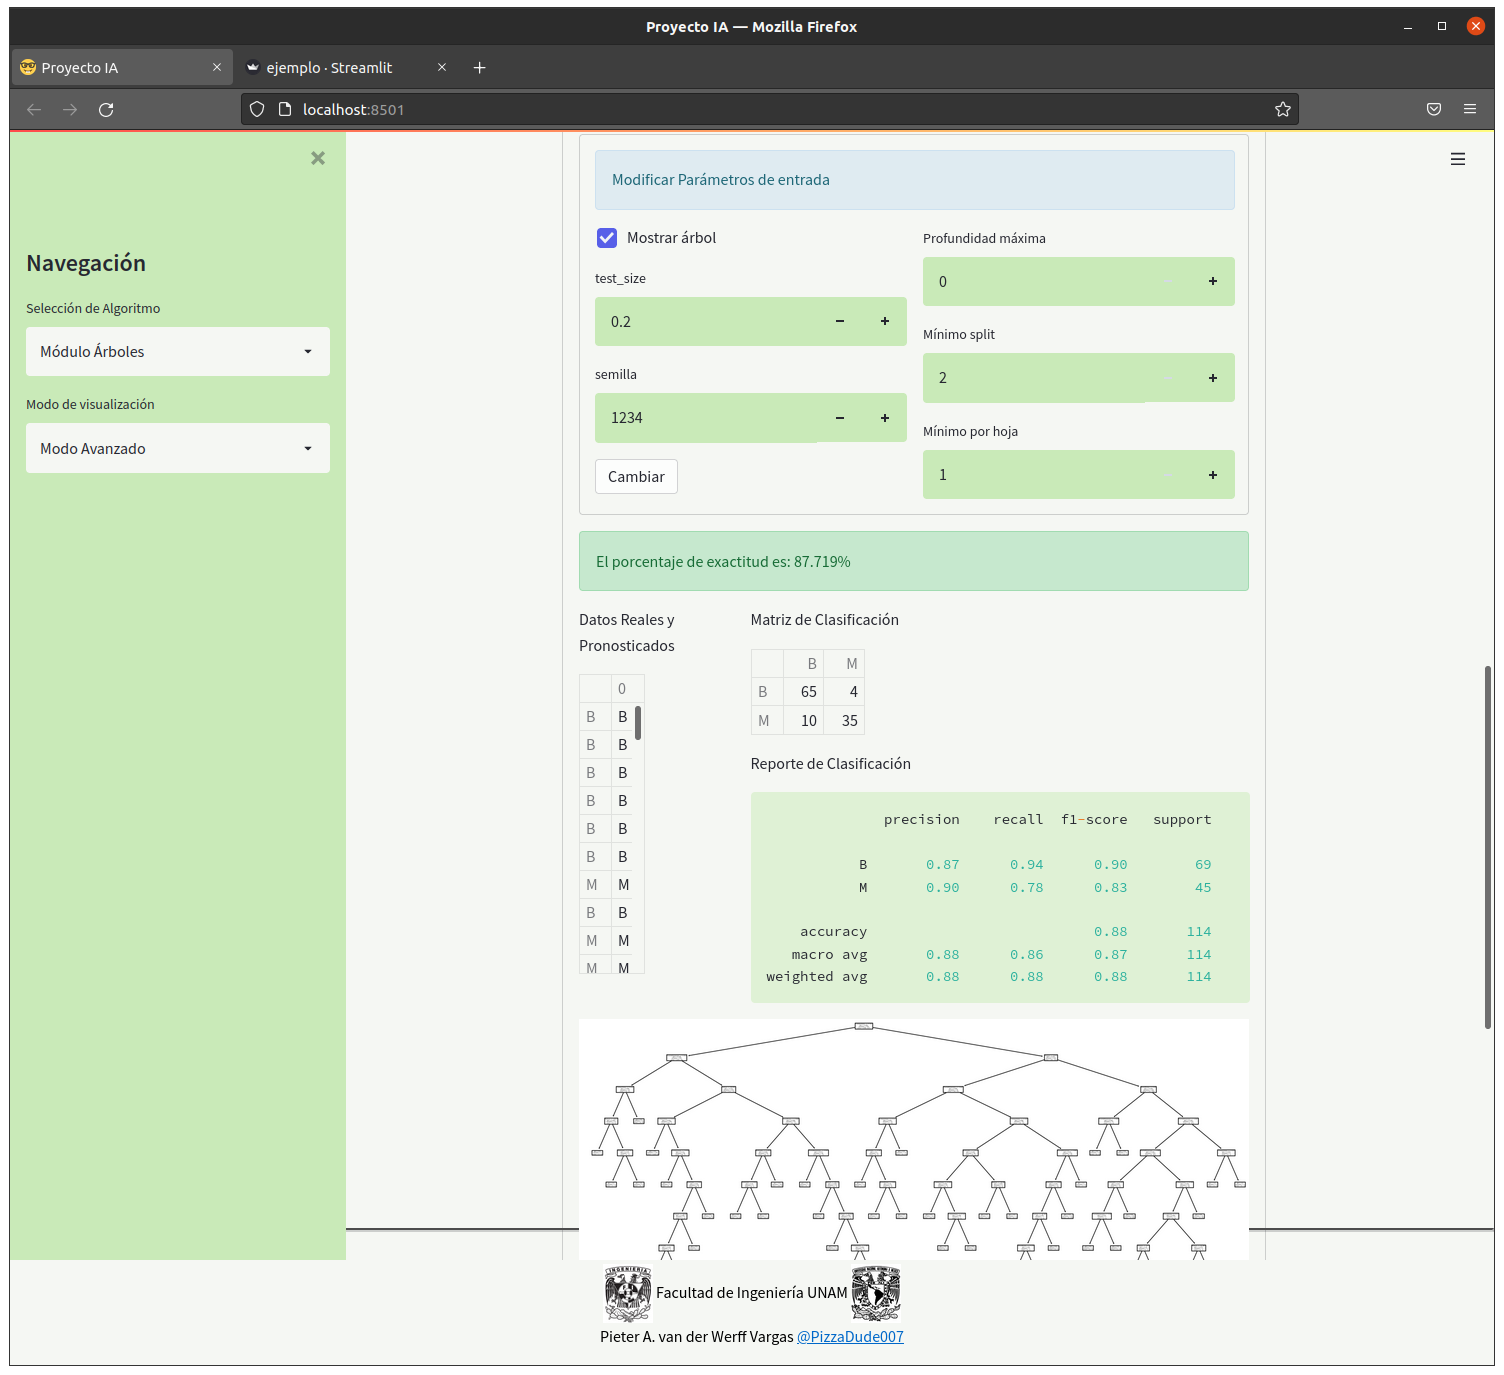
\includegraphics[height=6cm]{img/ÁrbolesClasificaciónMA.png} 
    \caption{Clasificación Modo Avanzado}
    \label{fig:ArbolMAc}
    \end{figure}
    
    Si se utiliza el \textit{Modo Avanzado} es posible alterar los parámetros con los cuales son creados el árbol para cada tipo de algoritmo, de forma que se puede obtener un mejor porcentaje de exactitud para el algoritmo y disminuir el sobre-ajuste que pudiera existir en el árbol generado. Para esto, es necesario también incluir una visualización gráfica del árbol, además de distintas métricas para medir el funcionamiento del algoritmo. En el caso del algoritmo de clasificación se muestra una matriz con una comparativa entre los datos reales y pronosticados, además de una matriz de clasificación y un reporte con la precisión y el soporte que tiene el algoritmo.\newline
    
    Para el caso del algoritmo de pronóstico, se visualiza además de la comparación entre datos reales y pronosticados el error medio cuadrático y otros parámetros que sean de utilidad para observar el funcionamiento del modelo generado por el árbol. Adicional a esto se muestra una matriz de importancia y una gráfica mostrando la comparación entre los datos reales y los calculados por el modelo.
    
    \begin{figure}[H]
    
    \begin{subfigure}{0.5\textwidth}
    \centering
    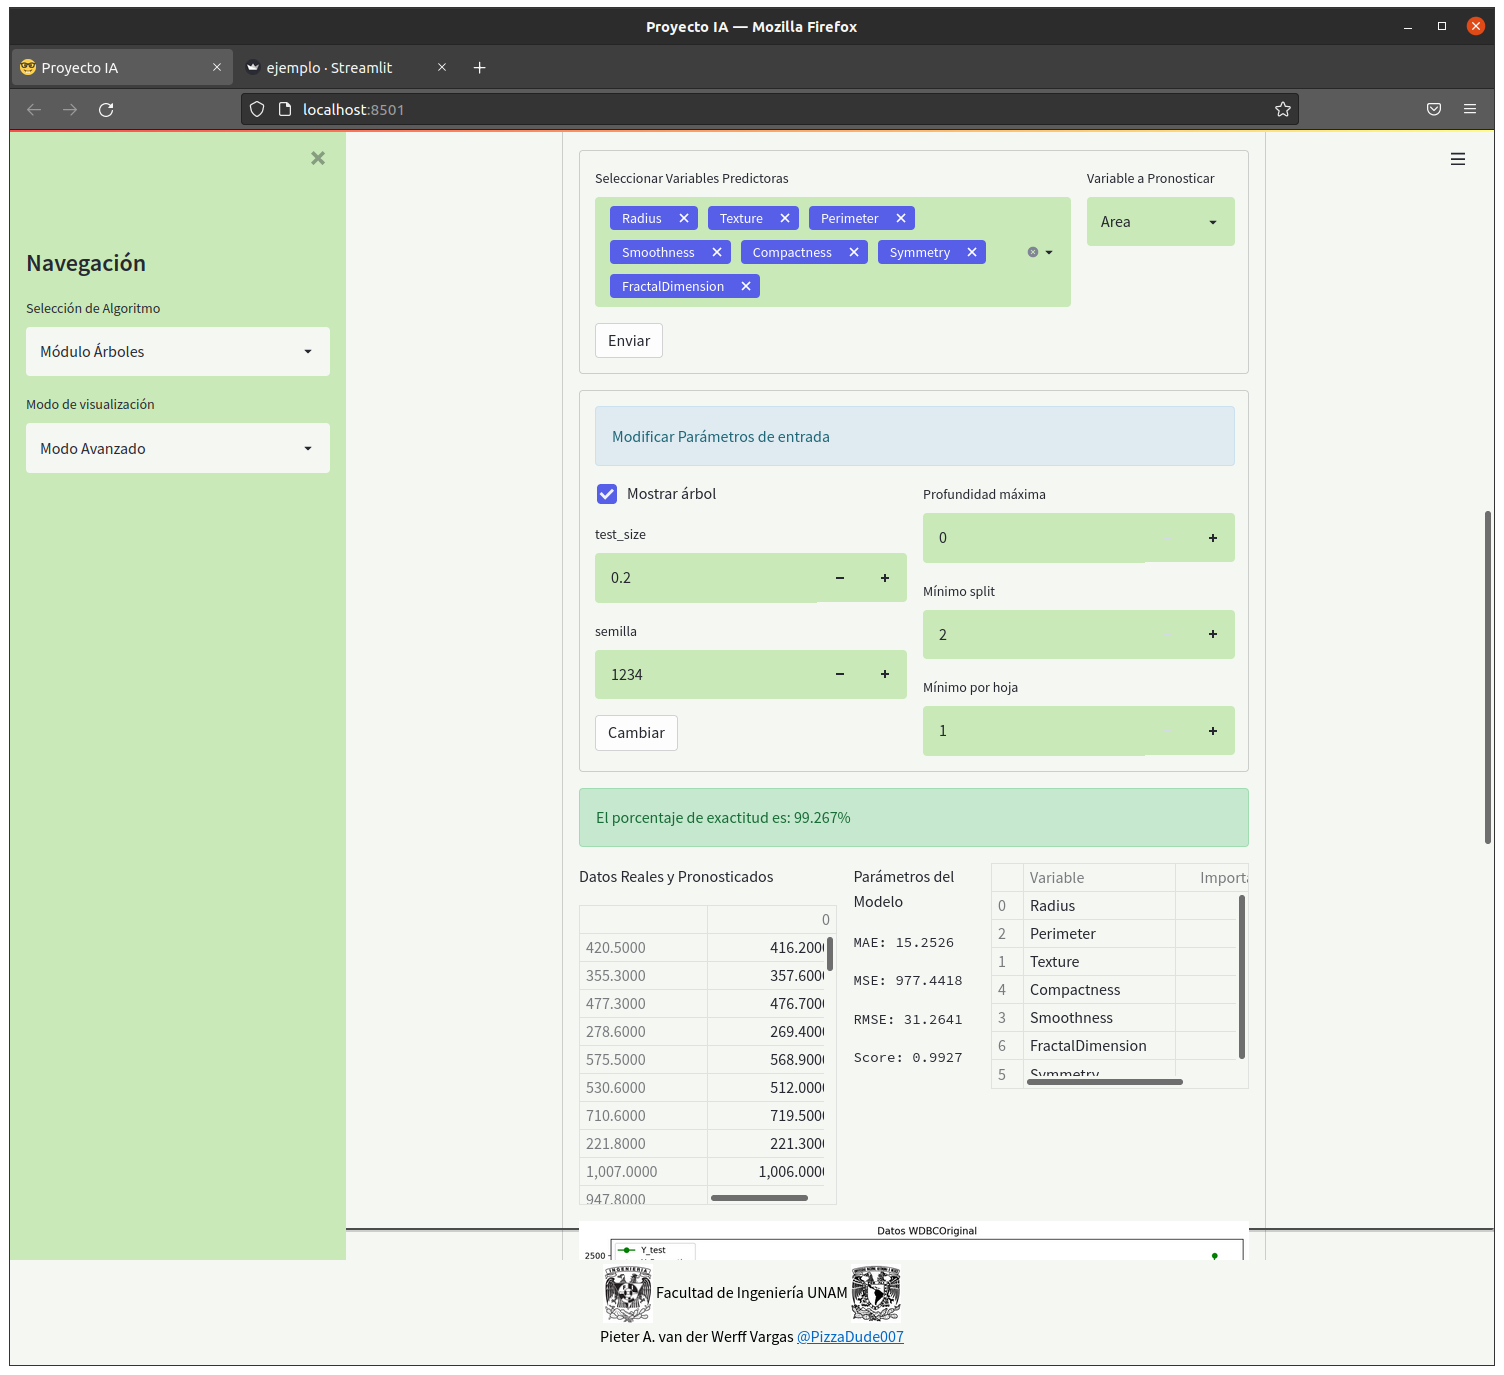
\includegraphics[height=6cm]{img/ÁrbolesPronósticoMA.png}
    \caption{Parámetros}
    \label{fig:ArbolMAp}
    \end{subfigure}
    \begin{subfigure}{0.5\textwidth}
    \centering
    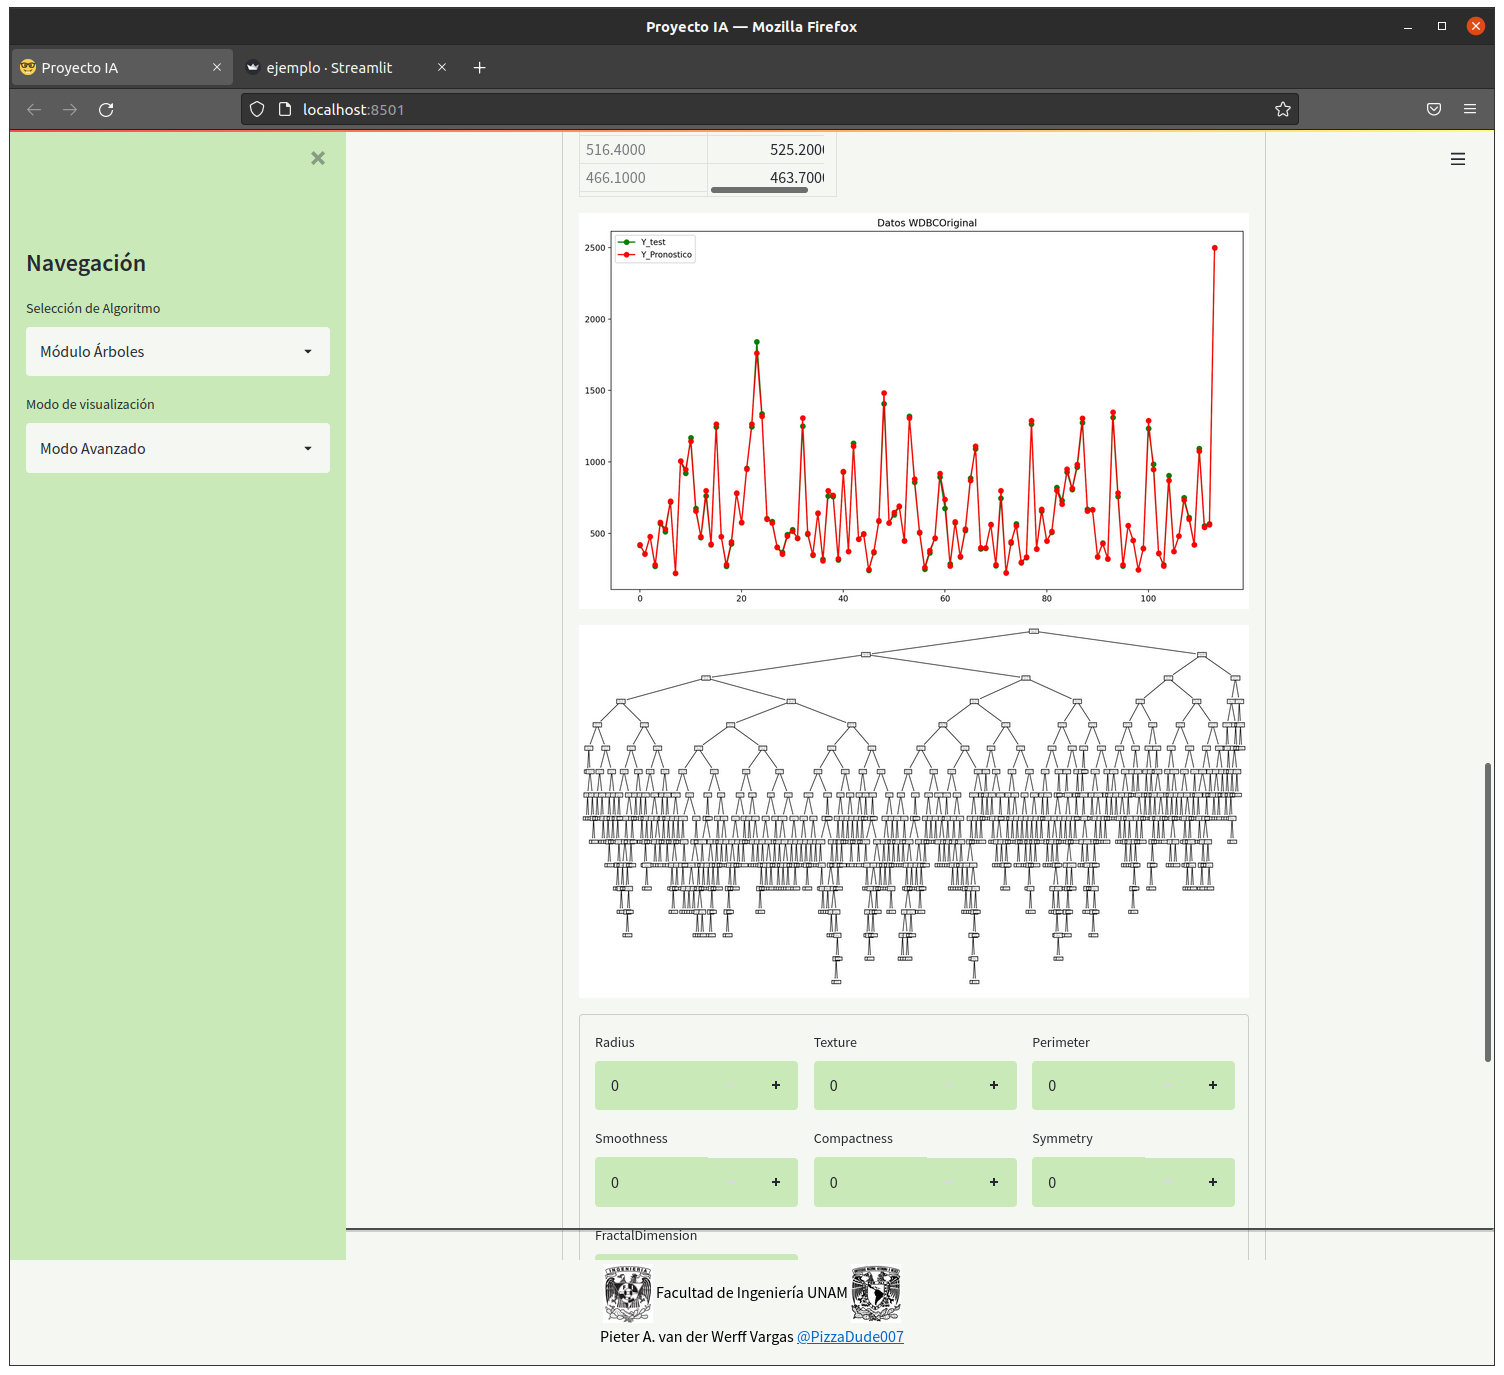
\includegraphics[height=6cm]{img/ÁrbolPronósticoMA_graficas.png}
    \caption{Gráficas}
    \label{fig:ArbolMAp2}
    \end{subfigure}
    
    \caption{Pronóstico Modo Avanzado}
    \label{fig:ArbolesMAparametros}
    \end{figure}
    
\section{Conclusión}
A lo largo del semestre observamos el comportamiento de distintos algoritmos de inteligencia artificial, de tipo supervisado y no supervisado. Es interesante observar que aplicaciones se tienen para cada uno de estos, que inclusive utilizamos en nuestro día a día sin estar al tanto de ello. Es por ello importante entender su funcionamiento y aplicaciones, lo cual se explica y ejemplifica con la realización de este proyecto. Se pudo, mediante una aplicación web basada en la herramienta Streamlit, desarrollar una forma de visualizar de manera sencilla el comportamiento y utilidad de cada uno de estos algoritmos, los cuales se explicaron de manera teórica en clase.


\end{document}
